\chapter{Inference for categorical data}
\label{inferenceForCategoricalData}

Chapter~\ref{foundationsForInference} introduced the logic and the steps for constructing confidence intervals and carrying out tests of hypothesis. We use these methods to answer questions like the following:
\begin{itemize}
\setlength{\itemsep}{0mm}
\item What proportion of the American public approves of the job the Supreme Court is doing?
\item The Pew Research Center conducted a poll about support for the 2010 health care law, and they used two forms of the survey question. Each respondent was randomly given one of the two questions. What is the difference in the support for respondents under the two question orderings?
\end{itemize}
The methods we learned in Chapter~\ref{foundationsForInference} are very useful in these settings. In this chapter we will consider the sampling distribution for a proportion and for the difference of two proportions, and we will examine the conditions under which a normal model is appropriate. We will also encounter a new distribution for hypothesis tests on frequency and contingency tables.



%__________________
\section{Inference for a single proportion}
\label{singleProportion}

The distribution of a sample proportion, such as an estimate of the fraction of people who share a particular opinion in a poll, was introduced in Section~\ref{distributionphat}.

\Comment{The first subsection felt awkward (no motivation for why that content was shown), so I merged the content within the example in the subsequent subsection.}

\subsection{Confidence intervals for a proportion}
\label{confIntForPropSection}

\index{data!supreme court|(}
\index{point estimate!single proportion}

Suppose we want to construct a confidence interval for the proportion of Americans who approve of the job the Supreme Court is doing. In a simple random sample of $n = 976$, 44\% of respondents approved.\footnote{\href{http://www.nytimes.com/2012/06/08/us/politics/44-percent-of-americans-approve-of-supreme-court-in-new-poll.html}{\scriptsize nytimes.com/2012/06/08/us/politics/44-percent-of-americans-approve-of-supreme-court-in-new-poll.html}} \Add{In the examples below, we will construct a \emph{1-proportion Z interval}.}


\Add{Before constructing the confidence interval, we should determine whether we can model the sample proportion, $\hat{p} = 0.44$, using a normal model, which requires two conditions to be satisfied.}

\Comment{David: this term box feels a bit redundant with the longer term box at the end of the section, and it also puts a lot of emphasis on checking conditions while we don't do anything like this for the other five steps in constructing a confidence interval. Basically, I'd favor cutting it and tweaking the text in Example~\ref{supremeCourtCIConditionsExample} to accommodate.}

\begin{termBox}{\tBoxTitle{Conditions for the sampling distribution of $\hat{p}$ being nearly normal}
The sampling distribution for $\hat{p}$, taken from a sample of size $n$ from a population with a true proportion $p$, is nearly normal when
\begin{enumerate}
\item the sample observations are independent and
\item we expected to see at least 10 successes and 10 failures in our sample, i.e. $np\geq10$ and $n(1-p)\geq10$. This is called the \term{success-failure condition}.
\end{enumerate}
If these conditions are met, then the sampling distribution of $\hat{p}$ is nearly normal with mean $\mu_{\hat{p}}=p$ and standard deviation $\sigma_{\hat{p}} = \sqrt{\frac{\ p(1-p)\ }{n}}$.\index{standard error!single proportion}}
\end{termBox}

\Add{\begin{example}{Verify that we can use a normal distribution to model $\hat{p}=0.44$ for the Supreme Court poll of $n = 976$ US adults.}
\label{supremeCourtCIConditionsExample}
The data are from a simple random sample, so the independence condition is satisfied. To check that $np$ and $n(1-p)$ are both at least 10, we will use the sample proportion in place of the population proportion:
\begin{align*}
np &\approx n\hat{p} = 976 \times 0.44 = 429\text{ (``successes'')} \\
n(1-p) &\approx n(1-\hat{p}) = 976 \times (1 - 0.44) = 547\text{ (``failures'')}
\end{align*}
The second condition is satisfied since 429 and 547 are both larger than 10. With the two conditions satisfied, we can model the sample proportion $\hat{p} = 0.44$ using a normal model.
\end{example}}

\begin{tipBox}{\tipBoxTitle{Reminder on checking independence of observations}
If data come from a simple random sample, then the independence assumption is generally reasonable. Alternatively, if the data come from a random process, we must evaluate the independence condition more carefully.}
\end{tipBox}

\begin{example}{The general form of a confidence interval is:
\begin{align*}
\text{point estimate}\ \pm\ \text{critical value} \times SE\vspace{-2mm}
\end{align*}
What should we use as the point estimate for the confidence interval?}
\label{supremeCourtCISEExample}
The best estimate for the unknown parameter $p$ (the proportion of Americans who approve of the job the Supreme Court is doing) is the sample proportion. When constructing a confidence interval for a single proportion, we use $\hat{p} = 0.44$ as the point estimate for $p$.
\end{example}

\begin{example}{Calculate the standard error for the confidence interval.}
\label{supremeCourtCIFinishedExample}
In Section~\ref{distributionphat}, we learned that the formula for the standard error of $\hat{p}$ is
\begin{align*}
\sigma_{\hat{p}} = \sqrt{\frac{\ p(1-p)\ }{n}}
\end{align*}
The proportion $p$ is unknown, but we can use sample proportion $\hat{p}$ instead when finding the SE in a confidence interval:
\begin{align*}
SE = \sqrt{\frac{0.44(1-0.44)}{976}}= 0.016
\end{align*}
\end{example}

When the conditions for a normal model are met, we use $z^\star$ for the critical value. An appropriate value for $z^\star$ can most easily be found in the $t$ table on page~\pageref{tDistributionTable} in the last~row~($\infty$), where the column corresponds to the desired confidence level.

\begin{example}{Construct a 90\% confidence interval for $p$, the proportion of Americans who approve of the job the Supreme Court is doing.}\label{90CIForJobSupremeCourtDoingExample}
Using the point estimate $\hat{p} = 0.44$ and standard error $SE = 0.16$ computed earlier, we can construct the confidence interval:
\begin{align*}
\text{point estimate}\ \pm&\  \text{critical value} \times SE \\
0.44\ \pm&\  1.65 \times 0.016 \\
(0.414&,\ 0.466)
\end{align*}
The critical value $z^{\star}$ was found by looking in the 90\% column in the $t$ table on page~\pageref{tDistributionTable}.

We are 90\% confident that the true proportion of Americans who approve of the job the Supreme Court is doing is between 41.4\% and 46.6\%. Because the entire interval is below 0.5, we have evidence that the true percent that approve is less than 50\%.
\end{example}

\index{data!supreme court|)}

%Before proceeding, we check the conditions. The data are based on a simple random sample of 976 people in the U.S. population, so independence is confirmed. We also check our minimum sample size conditions: there were approximately $976\times \hat{p}=429$ ``successes'' and $976\times (1-\hat{p})=547$ ``failures'' in the sample, both easily greater than~10.
%
%With the conditions met, we are assured that the sampling distribution of $\hat{p}$ is nearly normal. Next, a standard error for $\hat{p}$ is needed, and then we can employ the usual method to construct a confidence interval.
%
%\begin{exercise} \label{seOfPropOfAmericansJobApprovalOfSupremeCourt}
%Compute the standard error of $\hat{p}=0.44$ for the context of a confidence interval.\footnote{$SD = \sqrt{\frac{p(1-p)}{n}} \approx \sqrt{\frac{0.44(1-0.44)}{976}} = 0.016$}
%\end{exercise}

\begin{termBox}{\tBoxTitle{Constructing a confidence interval for a proportion}
A complete solution to a confidence interval question for a single proportion includes the following steps:
\begin{enumerate}
\setlength{\itemsep}{0mm}
\item State the name of the confidence interval being used.\vspace{-1.5mm}
\begin{itemize}
\item 1-proportion Z Interval
\end{itemize}
\item Verify \textbf{conditions}.\vspace{-1.5mm}
\begin{itemize}
\setlength{\itemsep}{0mm}
\item a simple random sample
\item $n\hat{p} \geq10$ and $n(1-\hat{p})\geq10$
\end{itemize}
\item Plug in the numbers and write the interval in the form\vspace{-1.5mm}
\begin{align*}
\text{point estimate } \pm \text{ critical value}\times \text{SE of estimate}
\end{align*}
\begin{itemize}
\item The point estimate is $\hat{p}$.
\item Plug in a critical value $z^\star$ (e.g. 1.96 for a 95\% CI).
\item Use $SE = \sqrt{\frac{\hat{p}(1-\hat{p})}{n}}$.
\end{itemize}
\item Evaluate the CI and write in the form (\underline{\ \ \ \ \ }, \underline{\ \ \ \ \ }).
\item Interpret the interval:  ``We are [XX]\% confident that the true proportion of [...] is between [...] and [...]."
\item State your conclusion to the original question.
\end{enumerate}}
\end{termBox}

\Add{
\begin{exercise}
Identify each of the six steps for constructing a confidence interval in the Supreme Court description and examples.\footnote{The following are the required components for constructing a confidence interval for a single proportion. 1.~The last sentence in the first paragraph of Section~\ref{confIntForPropSection}. 2.~in the solution to Example~\ref{supremeCourtCIConditionsExample}, the first sentence to cover independence and the two calculations verifying $n\hat{p}$ and $n(1-\hat{p})$ were at least 10. 3.~The last formula in the solution to Example~\ref{supremeCourtCIFinishedExample} and the calculations and identification of $z^{\star}$ in Example~\ref{supremeCourtCIFinishedExample}. 4.~At the end of the calculations in the solution to Example~\ref{supremeCourtCIFinishedExample}. Items~5 and~6 were contained in the last paragraph of Example~\ref{supremeCourtCISEExample}'s solution.}
\end{exercise}
}

\Comment{David: I moved the entire example to before the term box. Some of the earlier topics were also previously being covered out of order (e.g. omitted conditions) before the term box, so it felt a bit ironic to provide the structure described in the term box and not adhere to it within this section.

Ping Mine to get a second example to be used to show a fully-fleshed example without generalized explanations.}



\subsection{Hypothesis testing for a proportion}
\label{htForPropSection}

While a confidence interval provides a reasonable range of values for an unknown parameter, a hypothesis test evaluates a specific claim. In a hypothesis test, we declare what test we will use, check that the test is reasonable for the context, and construct appropriate null and alternative hypotheses. We then construct a p-value for the test and use it to assess the hypotheses, which allows us to form a conclusion based on the data.

\begin{example}{Deborah Toohey is running for Congress, and her campaign manager claims she has more than 50\% from the district's electorate. A newspaper collects a simple random sample of 500 likely voters in the district and estimates Toohey's support to be 52\%.
\begin{itemize}
\item[(a)] What is the name of the test that is appropriate for this context?
\item[(b)] Identify the value we should use as the null value, $p_{0}$.
\item[(c)] Can we model $\hat{p} = 0.52$ using a normal model? Check the conditions.
\end{itemize}}
\label{TooheyTestNameAndConditionExample}
(a) The name of the test we will use is the \emph{1-proportion Z test}. \\[2mm]
(b) The alternate hypothesis, the one that bears the burden of proof, argues that Toohey has more than 50\% support. Therefore, $H_A$ will be one sided and the null value will be $p_0 = 50\% = 0.5$. \\[2mm]
(c) The calculations in a hypothesis test for a proportion assume the value $p_0$ for the unknown $p$, so we use $p_{0}$ when verifying the hypothesis test conditions:
\begin{align*}
np_0 &\geq 10 \quad \rightarrow \quad 500\times 0.5 \geq 10 \\
n(1-p_0) &\geq 10 \quad \rightarrow \quad 500 \times (1-0.5) \geq 10
\end{align*}
The conditions for a normal model are met.
\end{example}

In Chapter~\ref{foundationsForInference}, we saw that the general form of the test statistic for a hypothesis test took the following form:
\begin{align*}
\text{test statistic} = \frac{\text{point estimate} - \text{null value}}{\text{SE of estimate}}
\end{align*}
When the conditions for a normal model are met,
\begin{itemize}
\item we use Z as the test statistic,
\item the point estimate is $\hat{p}$ (just like for a confidence interval), and
\item since we compute the test statistic under the null hypothesized value of $p = p_0$, we compute the standard error as
\begin{align*}
SE = \sqrt{\frac{p_0(1-p_0)}{n}}
\end{align*}
\end{itemize}

\begin{example}{Deborah Toohey is running for Congress, and her campaign manager claimed she has more than 50\% support from the district's electorate. A newspaper poll finds that 52\% of 500 likely voters who were sampled support Toohey. Does this provide convincing evidence for the claim by Toohey's manager at the 5\% significance level?}\label{TooheyInferenceExample}
We will use a one-sided test with the following hypotheses:
\begin{itemize}
\item[$H_0$:] $p = 0.5$. Toohey's support is 50\%.
\item[$H_A$:] $p > 0.5$. Toohey's manager is correct, and her support is higher than 50\%.
\end{itemize}
We will use a significance level of $\alpha = 0.05$ for the test. We can compute the standard error as
\begin{align*}
SE = \sqrt{\frac{0.5 (1 - 0.5)}{500}} = 0.022
\end{align*}
The test statistic can be computed as:
\begin{align*}
Z = \frac{0.52 - 0.50}{0.022} = 0.89
\end{align*}
A picture featuring the p-value is shown in Figure~\ref{pValueForCampaignManagerClaimOfMoreThan50PercentSupport} as the shaded region. Using a table or a calculator, we can get the p-value as about 0.19, which is larger than $\alpha = 0.05$, so we do not reject $H_0$. That is, we do not have strong evidence to support Toohey's campaign manager's claims that she has more than 50\% support within the district.
\end{example}

\begin{figure}[h]
\centering
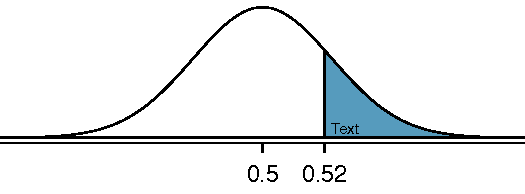
\includegraphics[width=0.5\textwidth]{ch_inference_for_props/figures/pValueForCampaignManagerClaimOfMoreThan50PercentSupport/pValueForCampaignManagerClaimOfMoreThan50PercentSupport}
\caption{Sampling distribution of the sample proportion if the null hypothesis is true for Example~\ref{TooheyInferenceExample}. The p-value for the test is shaded.}
\label{pValueForCampaignManagerClaimOfMoreThan50PercentSupport}
\end{figure}

\begin{termBox}{\tBoxTitle{Hypothesis test for a proportion}
A complete solution to a test of hypothesis problem for a single proportion should include the following steps:
\begin{enumerate}
\setlength{\itemsep}{0mm}
\item State the name of the test being used: 1-proportion Z test.
\item Verify conditions to ensure the standard error estimate is reasonable and the point estimate is nearly normal and unbiased.\vspace{-1.5mm}
  \begin{itemize}
  \setlength{\itemsep}{0mm}
  \item a simple random sample
  \item $np_0\geq10$ and $n(1-p_0)\geq10$
  \end{itemize}
\item Write the hypotheses in plain language and mathematical notation.\vspace{-1.5mm}
  \begin{itemize}
  \setlength{\itemsep}{0mm}
  \item H$_0: p = p_0$, where $p_0$ is the hypothesized value of $p$
  \item H$_A: p \ne \text{or} < \text{or} > p_0$
  \end{itemize}
\item Identify the significance level $\alpha$.
\vspace{-1.5mm}
\item Calculate the test statistic: $\text{Z} = \frac{\text{point estimate} - \text{null value}}{\text{SE of estimate}}$
  \begin{itemize}
  \item Use $\hat{p}$ as the point estimate, then use the null value $p_0$ for the standard error: $SE = \sqrt{\frac{p_0(1-p_0)}{n}}$.
  \end{itemize}
\item Find the p-value and compare it to $\alpha$ to determine whether to reject or not reject $H_0$.
\item Write the conclusion in the context of the question.
\end{enumerate}}
\end{termBox}

\begin{exercise}
Identify each of the seven steps for conducting a hypothesis test in the example for Toohey's support.\footnote{The following are the required components for running a hypothesis test for a single proportion. Items~1 and~2 are contained in Example~\ref{TooheyTestNameAndConditionExample}. Items~3-7 are covered in Example~\ref{TooheyInferenceExample}.}
\end{exercise}

\begin{exercise}
In Example~\ref{TooheyInferenceExample}, the data did not show strong evidence that Toohey's campaign manager was correct. Does this mean the manager was wrong?\footnote{Not necessarily. While we did not reject the null hypothesis, that does not mean it is true. It is possible that Toohey does have support above 50\%, but that the sample did not provide enough evidence to convincingly show this.}
\end{exercise}

\Comment{David: same overall change in this subsection as in the last subsection. If a complete run-through example is desired, we need another example. Leading with the generalization seems too formulaic.}


\subsection{Calculator: The 1-proportion Z test and CI\vspace{-3mm}}

We can use a calculator to compute a confidence interval or to evaluate the test statistic and the p-value. Remember to show work and first substitute in all numbers before using the calculator.

\Comment{TODO(David): add Casio calculator instructions.}

\begin{termBox}{\tBoxTitle{TI calculator: calculating the 1-proportion Z confidence interval}
Use \textbf{STAT, TESTS, 1-PropZInt}.
\begin{enumerate}
\setlength{\itemsep}{0mm}
\item Choose STAT.
\item Right arrow to TESTS.
\item Down arrow and choose A: 1-PropZInt.
\item Let x be the \emph{number} of yes's (must be an integer).
\item Let n be the sample size.
\item Let C-Level be the desired confidence level.
\item Choose Calculate and hit ENTER.
\begin{description}
\item[] This returns
\end{description}
\begin{tabular}{l l}
($\_$ , $\_$)
	&\quad  the confidence interval \\
$\hat{p}$
	&\quad	the sample proportion \\
n
	&\quad	the sample size
\end{tabular}
\end{enumerate}
}
\end{termBox}

\begin{exercise}
Using a calculator, confirm the earlier result from Example~\ref{90CIForJobSupremeCourtDoingExample}: a 90\% confidence interval for the percent of Americans who approve of the job the Supreme Court is doing is between 41.4\% and 47.1\%. The sample percent was 44\% and $n = 976$.
\end{exercise}

\begin{termBox}{\tBoxTitle{TI calculator: carrying out the 1-proportion Z test}
Use \textbf{STAT, TESTS, 1-PropZTest}.
\begin{enumerate}
\setlength{\itemsep}{0mm}
\item Choose STAT.
\item Right arrow to TESTS.
\item Down arrow and choose 5: 1-PropZTest.
\item Let p$_0$ be the null or hypothesized value of p.
\item Let x be the \emph{number} of yes's (must be an integer).
\item Let n be the sample size.
\item Choose $\ne$, $<$, or $>$ to correspond to H$_A$.
\item Choose Calculate and hit ENTER.
\begin{description}
\item[] This returns
\end{description}
\begin{tabular}{l l}
\text{z} &\quad  \text{Z statistic} \\
\text{p} &\quad  \text{p-value} \\
$\hat{p}$ &\quad  \text{the sample proportion} \\
\text{n} &\quad  \text{the sample size}
\end{tabular}
\end{enumerate}
}
\end{termBox}

%\CommentA{students will NOT look back in the text}
\begin{exercise}
Using a calculator, confirm the earlier result from Example~\ref{TooheyInferenceExample}, that we do not have strong evidence that Toohey's voter support is above 50\% because the p-value is 0.19. The sample percent was 52\% and $n=500$.
\end{exercise}


\subsection{Choosing a sample size when estimating a proportion}

\index{margin of error|(}

Planning a sample size before collecting data is important. If we collect too little data, the standard error of our point estimate may be so large that the data are not very useful. On the other hand, collecting data in some contexts is time-consuming and expensive, so we don't want to waste resources on collecting more data than we need.

\begin{example}{Suppose we are conducting a university survey to determine whether students support a \$200 per year increase in fees to pay for a new football stadium, how big of a sample is needed to be sure the margin of error is less than 0.04 using a 95\% confidence level? Find the smallest sample size $n$ so that the margin of error of the point estimate $\hat{p}$ will be no larger than $m=0.04$ when using a 95\% confidence interval.}
For a 95\% confidence level, the value $z^{\star}$ corresponds to 1.96, and we can write the margin of error expression as follows:
\begin{align*}
ME = 1.96 \times SE = 1.96\times \sqrt{\frac{p(1-p)}{n}} \leq 0.04
\end{align*}
There are two unknowns in the equation: $p$ and $n$. If we have an estimate of $p$, perhaps from a similar survey, we could use that value. If we have no such estimate, we must use some other value for $p$. It turns out that the margin of error is largest when $p$ is 0.5, so we typically use this \emph{worst case estimate} if no other estimate is available:
\begin{align*}
	1.96\times \sqrt{\frac{0.5(1-0.5)}{n}} &\leq 0.04 \\
	1.96^2\times \frac{0.5(1-0.5)}{n} &\leq 0.04^2 \\
	1.96^2\times \frac{0.5(1-0.5)}{0.04^2} &\leq n \\
	600.25 &\leq n \\
	n=601
\end{align*}
The sample size must be an integer and we round up because $n$ must be greater than or equal to 600.25. We need at least 601 participants to ensure the sample proportion is within 0.04 of the true proportion with 95\% confidence.
\end{example}

No estimate of the true proportion is required in sample size computations for a proportion. However, if we have an estimate of the proportion, we should use it in place of the worst case estimate of the proportion,~0.5.

\begin{exercise}
A manager is about to oversee the mass production of a new tire model in her factory, and she would like to estimate what proportion of these tires will be rejected through quality control. The quality control team has monitored the last three tire models produced by the factory, failing 1.7\% of tires in the first model, 6.2\% of the second model, and 1.3\% of the third model. The manager would like to examine enough tires to estimate the failure rate of the new tire model to within about 2\% with a 90\% confidence level.\footnote{(a)~For the 1.7\% estimate of $p$, we estimate the appropriate sample size as follows:
\begin{align*}
1.645\times \sqrt{\frac{0.017(1-0.017)}{n}} &\leq 0.02 \\
n &\geq 113.7 \\
n&=114
\end{align*}
Using the estimate from the first model, we would suggest examining 114 tires (round up!). A similar computation can be accomplished using 0.062 and 0.013 for $p$: 396 and 88. \par
(b) We could examine which of the old models is most like the new model, then choose the corresponding sample size. Or if two of the previous estimates are based on small samples while the other is based on a larger sample, we should consider the value corresponding to the larger sample. (Answers will vary.)}
\begin{itemize}
\setlength{\itemsep}{0mm}
\item[(a)] There are three different failure rates to choose from. Perform the sample size computation for each separately, and identify three sample sizes to consider.
\item[(b)] The sample sizes vary widely. Which of the three would you suggest using? What would influence your choice?
\index{margin of error|)}
\end{itemize}
\end{exercise}

\index{data!Congress approval rating|(}

\begin{exercise}
A recent estimate of Congress' approval rating was 17\%.\footnote{\href{http://www.gallup.com/poll/155144/Congress-Approval-June.aspx}{www.gallup.com/poll/155144/Congress-Approval-June.aspx}} What sample size does this estimate suggest we should use for a margin of error of 0.04 with 95\% confidence?\footnote{We complete the same computations as before, except now we use $0.17$ instead of $0.5$ for $p$:
\begin{align*}
1.96\times \sqrt{\frac{0.17(1-0.17)}{n}} \leq 0.04
\quad\rightarrow\quad
n \geq 338.8
\quad\rightarrow\quad
n = 339
\end{align*}
A sample size of 339 or more would be reasonable.}

\index{data!Congress approval rating|)}

\end{exercise}


%__________________
\section{Difference of two proportions}
\label{differenceOfTwoProportions}

We would like to make conclusions about the difference in two population proportions: $p_1 - p_2$. We consider three examples. In the first, we compare the approval of the 2010 healthcare law under two different question phrasings. In the second application, a company weighs whether they should switch to a higher quality parts manufacturer. In the last example, we examine the cancer risk to dogs from the use of yard herbicides.

In our investigations, we first identify a reasonable point estimate of $p_1 - p_2$ based on the sample. You may have already guessed its form: $\hat{p}_1 - \hat{p}_2$\index{point estimate!difference of proportions}. Next, we develop a formula for the standard deviation of $\hat{p}_1 - \hat{p}_2$.


\subsection{Sampling distribution of the difference of two proportions}

%\CommentA{added about mean and sd}
The mean or expected value of $\hat{p}_1 - \hat{p}_2$ is $p_1 - p_2$. The standard deviation can be computed as:
\begin{align*}
SD_{\hat{p}_1 - \hat{p}_2}
	= \sqrt{SD_{\hat{p}_1}^2 + SD_{\hat{p}_2}^2} 
	= \sqrt{\frac{p_1(1-p_1)}{n_1} + \frac{p_2(1-p_2)}{n_2}}
\end{align*}

In addition to the mean and the standard deviation of $\hat{p}_1 - \hat{p}_2$, we would like to the know the shape of its distribution. First, the sampling distribution for each sample proportion must be nearly normal, and secondly, the samples must be independent. Under these two conditions, the sampling distribution of $\hat{p}_1 - \hat{p}_2$ may be well approximated using the normal model.

%\CommentA{Changed to SD for consistency in naming}

\begin{termBox}{\tBoxTitle{Conditions for the sampling distribution of $\hat{p}_1 - \hat{p}_2$ to be normal}
The difference $\hat{p}_1 - \hat{p}_2$ tends to follow a normal model when
\begin{itemize}
\setlength{\itemsep}{0mm}
\item each proportion separately follows a normal model (check $n_1p_1 \geq 10$, $n_1(1-p_1) \geq 10$, $n_2p_2 \geq 10$, and $n_2(1-p_2) \geq 10$) and
\item the two samples are independent of each other.
\end{itemize}
The standard deviation of the difference in sample proportions is
\index{standard deviation!difference in proportions}
\begin{eqnarray}
SD_{\hat{p}_1 - \hat{p}_2}
	= \sqrt{\frac{p_1(1-p_1)}{n_1} + \frac{p_2(1-p_2)}{n_2}}
\label{sdForDiffOfProp}
\end{eqnarray}
where $p_1$ and $p_2$ represent the population proportions, and $n_1$ and $n_2$ represent the sample sizes.}
\end{termBox}


\subsection{Confidence Interval for $p_1 -p_2$}
%\subsection{Intervals and tests for $p_1 -p_2$}

In the setting of confidence intervals, the sample proportions are used in place of the population proportions to verify the success-failure condition and also compute standard error, just as was the case with a single proportion.

\begin{example}{The way a question is phrased can influence a person's response. For example, Pew Research Center conducted a survey with the following question:\footnote{\href{http://www.people-press.org/2012/03/26/public-remains-split-on-health-care-bill-opposed-to-mandate/}{www.people-press.org/2012/03/26/public-remains-split-on-health-care-bill-opposed-to-mandate/}. Sample sizes for each polling group are approximate.}
\begin{quote}
As you may know, by 2014 nearly all Americans will be required to have health insurance. [People who do not buy insurance will pay a penalty] while [People who cannot afford it will receive financial help from the government]. Do you approve or disapprove of this policy?
\end{quote}
\index{data!health care|(}For each randomly sampled respondent, the statements in brackets were randomized: either they were kept in the order given above, or the two statements were reversed. Table~\ref{pewPollResultsForRandomizedStatementOrdering} shows the results of this experiment. Create and interpret a 90\% confidence interval of the difference in approval.}

\begin{table}[t]
\centering
\begin{tabular}{p{50mm}c p{13mm}p{14mm}p{16.5mm}c}
	&\ & Sample size ($n_i$) & Approve law (\%)	& Disapprove law (\%)	& Other \\
\hline
``people who cannot afford it will receive financial help from the government'' is given second \vspace{2.5mm}
	& & 771	& 47	& 49	& 3 \\
``people who do not buy it will pay a penalty'' is given second
	& & 732	& 34	& 63	& 3 \\
\hline
\end{tabular}
\caption{Results for a Pew Research Center poll where the ordering of two statements in a question regarding healthcare were randomized.\vspaceB{-2mm}}
\label{pewPollResultsForRandomizedStatementOrdering}
\end{table}

First the conditions must be verified. Because each group is a simple random sample, the observations are independent, both within the samples and between the samples. The success-failure condition should also be verified:
\begin{align*}
771 \times 0.47 &\ge 10
	&771 \times 0.53 &\ge 10
	&732 \times 0.34 &\ge 10
	&732 \times 0.66 &\ge 10
\end{align*}
Because all conditions are met, the normal model can be used for the point estimate of the difference in support, where $p_1$ corresponds to the original ordering and $p_2$ to the reversed ordering:
$$\hat{p}_{1} - \hat{p}_{2} = 0.47 - 0.34 = 0.13$$
The standard error may be computed from Equation~\eqref{sdForDiffOfProp} using the sample proportions in place of the population proportions:
$$SE = \sqrt{\frac{0.47(1-0.47)}{771} + \frac{0.34(1-0.34)}{732}} = 0.025$$
For a 90\% confidence interval, we use $z^{\star} = 1.645$:
\begin{align*}
\text{point estimate} \ \pm\ z^{\star}SE
\quad\rightarrow\quad
0.13 \ \pm\ 1.645 \times  0.025
\quad\rightarrow\quad
(0.09, 0.17)
\end{align*}
We are 90\% confident that the approval rating for the 2010 healthcare law changes between 9\% and 17\% due to the ordering of the two statements in the survey question. Because the entire interval is positive, we have evidence that the approval rating \emph{increased}. The Pew Research Center reported that this modestly large difference suggests that the opinions of much of the public are still fluid on the health insurance mandate.
\index{data!health care|)}
\end{example}

\begin{termBox}{\tBoxTitle[]{Constructing a confidence interval for the difference of two proportion}
\begin{enumerate}
\setlength{\itemsep}{0mm}
\item State the name of the CI being used.
\begin{itemize}
\item 2 proportion Z Interval
\end{itemize}
\item Verify conditions.
\begin{itemize}
\item 2 independent random samples OR 2 randomly allocated treatments
\item $n_1\hat{p}_1\geq10$, $n_1(1-\hat{p}_1)\geq10$  \newline $n_2\hat{p}_2\geq10$, $n_2(1-\hat{p}_2)\geq10$
\end{itemize}
\item Plug in the numbers and write the interval in the form
$$\text{point estimate } \pm \text{ critical value}\times \text{SE of estimate}$$
\begin{itemize}
\item point estimate = $\hat{p}_1-\hat{p}_2$
\item critical value $Z^*$ = 1.96 for a 95\% CI\newline otherwise find $Z^*$ using the $t$~table at row $\infty$.
\item SE = $\sqrt{\frac{\hat{p}_1(1-\hat{p}_1)}{n_1} + \frac{\hat{p}_2(1-\hat{p}_2)}{n_2}}$
\end{itemize}
\item Evaluate the CI and write in the form (\underline{\ \ \ \ \ }, \underline{\ \ \ \ \ }).
\item Interpret the interval: ``We are [XX]\% confident that the true difference in the proportion of [...] is between [...] and [...].
\item State your conclusion to the original question.
\end{enumerate}}
\end{termBox}

\begin{example}{A remote control car company is considering a new manufacturer for wheel gears. The new manufacturer would be more expensive but their higher quality gears are more reliable, resulting in happier customers and fewer warranty claims. However, management must be convinced that the more expensive gears are worth the conversion before they approve the switch. The quality control engineer collects a sample of gears, examining 1000 gears from each company and finds that 899 gears pass inspection from the current supplier and 958 pass inspection from the prospective supplier. Using these data, construct a 95\% confidence interval for the difference in the proportion that pass inspection.}
We will calculate a 2 proportion Z Interval.

The samples are independent, but not necessarily random, so to proceed we must assume the gears are all independent. For this sample we will suppose this assumption is reasonable, but the engineer would be more knowledgeable as to whether this assumption is appropriate. We also must verify the minimum sample size conditions:
\begin{align*}
1000 \times \frac{899}{1000} &\ge 10
	&1000 \times \frac{101}{1000} &\ge 10
	&1000 \times \frac{958}{1000} &\ge 10
	&1000 \times \frac{42}{1000} &\ge 10
\end{align*}
To construct a confidence interval, we first identify the point estimate and standard error, then we can construct the confidence interval:
\begin{align*}
&\text{point estimate} = 0.958 - 0.899 = 0.059 \\
&SE = \sqrt{\frac{0.899(1-0.899)}{1000} +
			\frac{0.958(1-0.958)}{1000}}
	= 0.0114 \\
&0.059\ \pm\ 1.96 \times 0.0114 \\
&(0.037, 0.081)
\end{align*}
We are 95\% confident that the true difference in proportion of current and prospective gears that pass inspection is between 0.037 and 0.081, favoring the prospective gears. Because the entire interval is above zero, the data provide strong evidence that the prospective gears pass inspection more often than the current gears. The remote control car company should go with the new manufacturer.
\end{example}


\subsection{Hypothesis testing when $H_0: p_1 = p_2$}
\label{pooledHTForProportionsSection}

\index{data!cancer in dogs, herbicide|(}

Here we use a new example to examine a special estimate of the standard error when $H_0: p_1 = p_2$. We investigate whether there is an increased risk of cancer in dogs that are exposed to the herbicide 2,4-dichlorophenoxyacetic acid (2,4-D). A study in 1994 examined 491 dogs that had developed cancer and 945 dogs as a control group.\footnote{Hayes HM, Tarone RE, Cantor KP, Jessen CR, McCurnin DM, and Richardson RC. 1991. Case-Control Study of Canine Malignant Lymphoma: Positive Association With Dog Owner's Use of 2, 4-Dichlorophenoxyacetic Acid Herbicides. Journal of the National Cancer Institute 83(17):1226-1231.} Of these two groups, researchers identified which dogs had been exposed to 2,4-D in their owner's yard. The results are shown in Table~\ref{24DAndCancerInDogs}.

\begin{table}[h]
\centering
\begin{tabular}{rrr}
  \hline
 & cancer & no cancer \\
  \hline
2,4-D & 191 & 304 \\
no 2,4-D & 300 & 641 \\
   \hline
\end{tabular}
\caption{Summary results for cancer in dogs and the use of 2,4-D by the dog's owner.}
\label{24DAndCancerInDogs}
\end{table}

\begin{exercise}
Is this study an experiment or an observational study?\footnote{The owners were not instructed to apply or not apply the herbicide, so this is an observational study. This question was especially tricky because one group was called the \emph{control group}, which is a term usually seen in experiments.}
\end{exercise}

\begin{exercise}\label{htFor24DAndCancerInDogs}
Set up hypotheses to test whether 2,4-D and the occurrence of cancer in dogs are related. Use a one-sided test and compare across the cancer and no cancer groups.%
\footnote{Using the proportions within the cancer and no cancer groups may seem odd. We intuitively may desire to compare the fraction of dogs with cancer in the 2,4-D and no 2,4-D groups, since the herbicide is an explanatory variable. However, the cancer rates in each group do not necessarily reflect the real cancer rates due to the way the data were collected. For this reason, computing cancer rates may greatly alarm dog owners. \\ $H_0$: the proportion of dogs with exposure to 2,4-D is the same in ``cancer'' and ``no cancer'' dogs, $p_c - p_n = 0$. \\ $H_A$: dogs with cancer are more likely to have been exposed to 2,4-D than dogs without cancer, $p_c - p_n > 0$.}
\end{exercise}

\begin{example}{Are the conditions for using the normal model and make inference on the results?}\label{condFor24DAndCancerInDogsNormalInference}
(1) It is unclear whether this is a random sample. However, if we believe the dogs in both the cancer and no cancer groups are representative of each respective population and that the dogs in the study do not interact in any way, then we may find it reasonable to assume independence between observations. (2) The success-failure condition (minimums of 10) easily holds for each sample.

Under the assumption of independence, we can use the normal model and make statements regarding the canine population based on the data.
\end{example}

%\CommentA{Called term SD rather than SE to be consistent with notation and with language used in paragraph.}

In the hypotheses for Guided Practice~\ref{htFor24DAndCancerInDogs}, the null is that the proportion of dogs with exposure to 2,4-D is the same in each group. The point estimate of the difference in sample proportions is $\hat{p}_c - \hat{p}_n = 0.067$. To identify the p-value for this test, we first check conditions (Example~\ref{condFor24DAndCancerInDogsNormalInference}) and compute the standard error of the difference. 

The standard deviation is given by
\begin{align*}
SD = \sqrt{\frac{p_c(1-p_c)}{n_c} + \frac{p_n(1-p_n)}{n_n}}
\end{align*}
In a hypothesis test, the distribution of the test statistic is always examined as though the null hypothesis is true, i.e. in this case, $p_c = p_n$. The standard deviation formula should reflect this equality in the null hypothesis. We will use $p$ to represent the common rate of dogs that are exposed to 2,4-D in the two groups:
\begin{align*}
SD &= \sqrt{\frac{p(1-p)}{n_c} + \frac{p(1-p)}{n_n}} \\
	&= \sqrt{p(1-p)}\sqrt{\frac{1}{n_c} + \frac{1}{n_n}}
\end{align*}
We don't know the exposure rate, $p$, but we can obtain a good estimate of it by \emph{pooling} the results of both samples to find $\hat{p}$:
$$\hat{p} = \frac{\text{\# of ``successes''}}{\text{\# of cases}} = \frac{191 + 304}{191+300+304+641} = 0.345$$
This is called the \term{pooled estimate} of the sample proportion, and we use it to compute the standard error when the null hypothesis is that $p_1 = p_2$ (e.g. $p_c = p_n$ or $p_c - p_n = 0$). We also typically use it to verify the success-failure condition.

\begin{termBox}{\tBoxTitle{Pooled estimate of a proportion}
When the null hypothesis is $p_1 = p_2$, it is useful to find the pooled estimate of the shared proportion:
\begin{eqnarray*}
\hat{p} = \frac{\text{number of ``successes''}}{\text{number of cases}} = \frac{x_1+x_2}{n_1+n_2}=\frac{\hat{p}_1n_1 + \hat{p}_2n_2}{n_1 + n_2}
\end{eqnarray*}
Here $x_1$ represents the number of successes in sample 1. $x_1$ can be computed as $\hat{p}_1n_1$ if it is unknown. Similarly, $x_2$ represents the number of successes in sample~2. It also can be computed as $\hat{p}_2n_2$.}
\end{termBox}

\begin{tipBox}{\tipBoxTitle{Use the pooled proportion estimate when $\mathbf{H_0: p_1 = p_2}$}
When the null hypothesis suggests the proportions are equal, we use the pooled proportion estimate ($\hat{p}$) to verify the success-failure condition and also to estimate the standard error:
\begin{eqnarray}
SE =\sqrt{\hat{p}(1-\hat{p})}\sqrt{\frac{1}{n_1} + \frac{1}{n_2}}
\label{seOfDiffInPropUsingPooledEstimate}
\end{eqnarray}}
\index{data!cancer in dogs, herbicide|)}
\end{tipBox}

\begin{exercise}\label{verifySEOfPooledEstimateOf24DWithCancerNoCancerDogs}
Using Equation~\eqref{seOfDiffInPropUsingPooledEstimate}, $\hat{p}=0.345$, $n_1 = 491$, and $n_2=945$, verify the estimate for the standard error in the context of a hypothesis test is $SE = 0.026$.
\end{exercise}

\begin{example}{Complete the hypothesis test using a significance level of 0.01.}
We will complete a 2-proportion Z test. The conditions are met  - we will assume that there two independent random samples. Using the pooled proportion:
\begin{align*}
n_1\hat{p} &= 491 \times 0.345 = 169.4
	& n_1(1 - \hat{p}) &= 491 \times 0.655 = 321.6 \\
n_2\hat{p} &= 945 \times 0.345 = 326
	& n_2(1 - \hat{p}) &= 945 \times 0.655 = 619
\end{align*}
are all at least 10. Now we set up hypotheses, which were identified in Guided Practice~\ref{htFor24DAndCancerInDogs}:
\begin{itemize}
\item[$H_0$:] The proportion of dogs with exposure to 2,4-D is the same in ``cancer'' and ``no cancer'' dogs, $p_c - p_n = 0$.
\item[$H_A$:] Dogs with cancer are more likely to have been exposed to 2,4-D than dogs without cancer, $p_c - p_n > 0$.
\end{itemize}
We will use a significance level of $\alpha = 0.01$. All values are much larger than 10. Under the assumption that there were two independent random samples, we can proceed.

Next, we compute the test statistic using the standard error using the result of Guided Practice~\ref{verifySEOfPooledEstimateOf24DWithCancerNoCancerDogs}:
\begin{eqnarray*}
Z = \frac{\text{point estimate} - \text{null value}}{SE} = \frac{0.067 - 0}{0.026} = 2.58
\end{eqnarray*}
Looking up $Z=2.58$ in the normal probability table: 0.9951. However this is the lower tail, and the upper tail represents the p-value: $1-0.9951 = 0.0049$. Because the p-value is smaller than $\alpha = 0.01$, we reject the null hypothesis and conclude that there is an association between dogs getting cancer and owners using 2,4-D.
\end{example}
 
\begin{termBox}{\tBoxTitle[]{Hypothesis test for the difference of two proportions}
\begin{enumerate}
\setlength{\itemsep}{0mm}
\item State the name of the test being used: 2-proportion Z test.
\item Verify conditions: (a)~2~independent random samples OR 2 randomly allocated treatments. (b)~Calculate the pooled sample proportion $\hat{p}$ and verify $n_1\hat{p}$, $n_2\hat{p}$, $n_1(1 - \hat{p})$, and $n_2(1 - \hat{p})$ are greater than or equal to 10.
\item Write the hypotheses in plain language, then set them up in mathematical notation, e.g. $H_0: p_1 - p_2 = 0$.
\item Identify the significance level $\alpha$.
\item Calculate the test statistic: $\text{Z} = \frac{(\hat{p}_1 - \hat{p}_2) - \text{null difference}}{SE}$. In this book, the null difference is always zero, and the standard error is given by\vspace{-3.5mm}
\begin{align*}
SE = \sqrt{\hat{p}(1-\hat{p})}\sqrt{\frac{1}{n_1} + \frac{1}{n_2}}
\end{align*}
\item Find the p-value and compare it to $\alpha$ to determine whether to reject or not reject $H_0$.
\item Write the conclusion in the context of the question.
\end{enumerate}}
\end{termBox}

%\begin{center}
%\begin{tabular}{p{50mm}c p{13mm}p{14mm}p{16.5mm}c}
%	&\ & Sample size ($n_i$) & Approve law (\%)	& Disapprove law (\%)	& Other \\
%\hline
%``people who cannot afford it will receive financial help from the government'' is given second \vspace{2.5mm}
%	& & 771	& 47	& 49	& 3 \\
%``people who do not buy it will pay a penalty'' is given second
%	& & 732	& 34	& 63	& 3 \\
%\hline
%\end{tabular}
%\end{center}
%
%\begin{example}{Look again at the survey conducted by the Pew Research Center. Carry out a two sided test of hypothesis at the 5\% significance level to determine if there was a significant difference in the proportion that approved based on the two different wordings.}
%Let first question be 1 and second question be 2.
%\begin{itemize}
%\item  We will conduct a 2 proportion Z test.
%\item H$_0$: $p_1=p_2$ \newline H$_A: p_1 \ne p_2$
%\item $\alpha=0.05$
%\item There were two independent random samples.
%\newline \newline $\hat{p}=\frac{0.47(771)+0.34(732)}{771+732}=0.407$ \newline \newline $771(0.407)\ge 10$, $771(1-0.47)\ge 10$ \newline $732(0.407)\ge 10$, $732(1-0.407)\ge 10$
%\item $Z=\frac{(0.47-0.37) - 0}{\sqrt{0.407(1-0.407}\sqrt{\frac{1}{771}+\frac{1}{732}}}=5.1$
%\item p-value $ =3.34\times 10^{-7} < \alpha$
%\item Reject H$_0$. There is evidence of a significant differences in the proportion of yes responses based on the wording of the question.
%\end{itemize}
%\end{example}


\subsection{Calculator: The 2 proportion Z test and CI\vspace{-3mm}}

\begin{termBox}{\tBoxTitle{TI calculator: Calculating the 2 proportion Z confidence interval}
Use \textbf{STAT, TESTS, 2-PropZInt}.
\begin{enumerate}
\setlength{\itemsep}{0mm}
\item Choose STAT.
\item Right arrow to TESTS.
\item Down arrow and choose B: 2-PropZInt.
\item Let x1 be the \emph{number} of yes's (must be an integer) in sample 1 and let n1 be the size of sample 1.
\item Let x2 be the \emph{number} of yes's (must be an integer) in sample 2 and let n2 be the size of sample 2.
\item Let C-Level be the desired confidence level.
\item Choose Calculate and hit ENTER, which returns: \\
\begin{tabular}{l ll ll}
\hspace{3mm}&
(\underline{\ \ \ }, \underline{\ \ \ })
	&\quad  the confidence interval \\
&
$\hat{p}_1$
	&\quad  sample 1 proportion
	&\quad	$n_1$
	&\quad  size of sample 1 \\
&
$\hat{p}_2$
	&\quad  sample 2 proportion
	&\quad	$n_2$
	&\quad  size of sample 2
\end{tabular}
\end{enumerate}
}
\end{termBox}

\begin{exercise}{Use the data in Table~\ref{24DAndCancerInDogsTableInCalcSection} and a calculator to find a 95\% confidence interval for the difference in proportion of dogs with cancer that have been exposed to 2,4-D versus not exposed to 2,4-D.}\footnote{Use STAT, TESTS, 2-PropZInt. Let x1 be 191 and n1 be $191+304$. Let x2 be 300 and n2 be $300+641$. Let C-Level be 0.95 and Calculate. The interval is (0.01484, 0.11926). Note that there is no value given for the pooled proportion since we do not pool for confidence intervals.}
\end{exercise}

\begin{table}[h]
\centering
\begin{tabular}{rrr}
  \hline
 & cancer & no cancer \\
  \hline
2,4-D & 191 & 304 \\
no 2,4-D & 300 & 641 \\
   \hline
\end{tabular}
\caption{Summary results for cancer in dogs and the use of 2,4-D by the dog's owner.}
\label{24DAndCancerInDogsTableInCalcSection}
\end{table}

\begin{termBox}{\tBoxTitle{TI calculator: Carrying out the 2 proportion Z test}
Use \textbf{STAT, TESTS, 2-PropZTest}.
\begin{enumerate}
\setlength{\itemsep}{0mm}
\item Choose STAT.
\item Right arrow to TESTS.
\item Down arrow and choose 6: 2-PropZTest.
\item Let x1 be the \emph{number} of yes's (must be an integer) in sample 1 and let n1 be the size of sample 1.
\item Let x2 be the \emph{number} of yes's (must be an integer) in sample 2 and let n2 be the size of sample 2.
\item Choose $\ne$, $<$, or $>$ to correspond to H$_A$.
\item Choose Calculate and hit ENTER, which returns:\\
\begin{tabular}{l ll ll}
\hspace{3mm}&
\text{z}
	&\quad  Z statistic
	&\quad	$p$
	&\quad  p-value \\
&
$\hat{p}_1$
	&\quad  sample 1 proportion
	&\quad	$\hat{p}$
	&\quad  pooled sample proportion \\
&
$\hat{p}_2$
	&\quad  sample 2 proportion
\end{tabular}
\end{enumerate}}
\end{termBox}

\begin{exercise}{Use the data in Table~\ref{24DAndCancerInDogsTableInCalcSection} and a calculator to find the Z score and p-value for one sided test with H$_A$: dogs with cancer are more likely to have been exposed to 2,4-D than dogs without cancer, $p_c - p_n > 0$.}\footnote{Use STAT, TESTS, 2-PropZTest. Let x1 be 191 and n1 be $191+304$. Let x2 be 300 and n2 be $300+641$. Choose $>$ and Calculate. $Z=2.55$ and p-value$=0.0055$. Also the pooled proportion $\hat{p}=0.342$.}
\end{exercise}



%__________________
\section{Testing for goodness of fit using chi-square}
\label{oneWayChiSquare}

In this section, we develop a method for assessing a null model when the data are binned.
This technique is commonly used in two circumstances:
\begin{itemize}
\setlength{\itemsep}{0mm}
\item Given a sample of cases that can be classified into several groups, determine if the sample is representative of the general population.
\item Evaluate whether data resemble a particular distribution, such as a normal distribution or a geometric distribution.
\end{itemize}
Each of these scenarios can be addressed using the same statistical test: a chi-square test.

\index{data!racial make-up of jury|(}

In the first case, we consider data from a random sample of 275 jurors in a small county. Jurors identified their racial group, as shown in Table~\ref{juryRepresentationAndCityRepresentationForRace}, and we would like to determine if these jurors are racially representative of the population. If the jury is representative of the population, then the proportions in the sample should roughly reflect the population of eligible jurors, i.e. registered voters.

\begin{table}[h]
\centering
\begin{tabular}{ll ccc c ll}
\hline
Race	 & \hspace{2mm} & White & Black & Hispanic & Other & \hspace{2mm} & Total \\
\hline
Representation in juries &	& 205 & 26 & 25 & 19 & & 275 \\
Registered voters	 & 		& 0.72 & 0.07 & 0.12 & 0.09 & & 1.00 \\
\hline
\end{tabular}
\caption{Representation by race in a city's juries and population.}
\label{juryRepresentationAndCityRepresentationForRace}
\end{table}

While the proportions in the juries do not precisely represent the population proportions, it is unclear whether these data provide convincing evidence that the sample is not representative. If the jurors really were randomly sampled from the registered voters, we might expect small differences due to chance. However, unusually large differences may provide convincing evidence that the juries were not representative.

A second application, assessing the fit of a distribution, is presented at the end of this section. Daily stock returns from the S\&P500 for the years 1990-2011 are used to assess whether stock activity each day is independent of the stock's behavior on previous days.

In these problems, we would like to examine all bins simultaneously, not simply compare one or two bins at a time, which will require us to develop a new test statistic.


\subsection{Creating a test statistic for one-way tables}

\begin{example}{Of the people in the city, 275 served on a jury. If the individuals are randomly selected to serve on a jury, about how many of the 275 people would we expect to be white? How many would we expect to be black?}
About 72\% of the population is white, so we would expect about 72\% of the jurors to be white: $0.72\times 275 = 198$.

Similarly, we would expect about 7\% of the jurors to be black, which would correspond to about $0.07\times 275 = 19.25$ black jurors.
\end{example}

\begin{exercise}
Twelve percent of the population is Hispanic and 9\% represent other races. How many of the 275 jurors would we expect to be Hispanic or from another race? Answers can be found in Table~\ref{expectedJuryRepresentationIfNoBias}.
\end{exercise}

\begin{table}[h]
\centering
\begin{tabular}{ll ccc c ll}
\hline
Race	 & \hspace{2mm} & White & Black & Hispanic & Other & \hspace{2mm} & Total \\
\hline
Observed data			&	& 205 & 26	& 25 & 19	&	& 275 \\
Expected counts	 &	& 198 & 19.25 & 33 & 24.75 & & 275 \\
\hline
\end{tabular}
\caption{Actual and expected make-up of the jurors.}
\label{expectedJuryRepresentationIfNoBias}
\end{table}

The sample proportion represented from each race among the 275 jurors was not a precise match for any ethnic group. While some sampling variation is expected, we would expect the sample proportions to be fairly similar to the population proportions if there is no bias on juries. We need to test whether the differences are strong enough to provide convincing evidence that the jurors are not a random sample. These ideas can be organized into hypotheses:
\begin{itemize}
\setlength{\itemsep}{0mm}
\item[$H_0$:] The jurors are a random sample, i.e. there is no racial bias in who serves on a jury, and the observed counts reflect natural sampling fluctuation.
\item[$H_A$:] The jurors are not randomly sampled, i.e. there is racial bias in juror selection.
\end{itemize}
To evaluate these hypotheses, we quantify how different the observed counts are from the expected counts. Strong evidence for the alternative hypothesis would come in the form of unusually large deviations in the groups from what would be expected based on sampling variation alone.


\subsection{The chi-square test statistic}
\label{chiSquareTestStatistic}

In previous hypothesis tests, we constructed a test statistic of the following form:
$$ Z = \frac{\text{point estimate} - \text{null value}}{\text{SE of point estimate}} $$
This construction was based on (1) identifying the difference between a point estimate and an expected value if the null hypothesis was true, and (2) standardizing that difference using the standard error of the point estimate. These two ideas will help in the construction of an appropriate test statistic for count data.

In this example we have four categories: white, black, hispanic, and other. Because we have four values rather than just one or two, we need a new tool to analyze the data. Our strategy will be to find a test statistic that measures the overall deviation between the observed and the expected counts. We first find the difference between the observed and expected counts for the four groups:
\begin{align*}
&&\text{White} && \text{Black} && \text{Hispanic} && \text{Other} \\
\text{observed - expected }&& 205-198 && 26-19.25
	&& 25-33
	&& 19-24.75
\end{align*}
Next, we square the differences:
\begin{align*}
&&\text{White} && \text{Black} && \text{Hispanic} && \text{Other} \\
\text{(observed - expected)}^2 && (205-198)^2 && (26-19.25)^2
	&& (25-33)^2
	&& (19-24.75)^2
\end{align*}
We must standardize each term. To know whether the squared difference is large, we compare it to what was expected. If the expected count was 5, a squared difference of 25 is very large. However, if the expected count was 1,000, a squared difference of 25 is very small. We will divide each of the squared differences by the corresponding expected count.
\begin{align*}
&&\text{White} && \text{Black} && \text{Hispanic} && \text{Other} \\
\frac{\text{(observed - expected)}^2}{\text{expected}} && \frac{(205-198)^2}{198} && \frac{(26-19.25)^2 }{19.25}
	&& \frac{(25-33)^2}{33}
	&& \frac{(19-24.75)^2}{24.75}
\end{align*}
Finally, to arrive at the overall measure of deviation between the observed counts and the expected counts, we add up the terms.
\begin{align*}
X^2 &= \sum{\frac{\text{(observed - expected)}^2}{\text{expected}}} \\
	&= \frac{(205-198)^2}{198}
		+ \frac{(26-19.25)^2 }{19.25}
		+ \frac{(25-33)^2}{33}
		+ \frac{(19-24.75)^2}{24.75}
\end{align*}
%\Comment{The following sentence: The test statistic chii-sq is generally used for these reasons seems out of place. What reasons?}
% David: I am guessing the explanations were cut out during the development of the Preliminary Edition, but this sentence was accidentally left in.
We can write an equation for $X^2$\marginpar[\raggedright\vspace{9mm}

$X^2$\vspace{0.5mm}\\\footnotesize chi-square\\test statistic]{\raggedright\vspace{9mm}

$X^2$\vspace{0.5mm}\\\footnotesize chi-square\\test statistic} using the observed counts and expected counts:
\index{data!racial make-up of jury|)}
{\begin{align*}
X^2 &=
	\frac
	{\text{\footnotesize$(\text{observed count}_1 - \text{expected count}_1)^2$}}
	{\text{\footnotesize$\text{expected count}_1$}}
	+ \dots + \frac
	{\text{\footnotesize$(\text{observed count}_4 - \text{expected count}_4)^2$}}
	{\text{\footnotesize$\text{expected count}_4$}}
\end{align*}
}The final number $X^2$ summarizes how strongly the observed counts tend to deviate from the null counts.

In Section~\ref{pValueForAChiSquareTest}, we will see that if the null hypothesis is true, then $X^2$ follows a new distribution called a \emph{chi-square distribution}. Using this distribution, we will be able to obtain a p-value to evaluate whether there appears to be racial bias in the juries for the city we are considering.


\subsection{The chi-square distribution and finding areas}

The \term{chi-square distribution} is sometimes used to characterize data sets and statistics that are always positive and typically right skewed. Recall the normal distribution had two parameters -- mean and standard deviation -- that could be used to describe its exact characteristics. The chi-square distribution has just one parameter called \termsub{degrees of freedom (df)}{degrees of freedom (df)!chi-square}, which influences the shape, center, and spread of the distribution.

\begin{exercise}\label{exerChiSquareDistributionDescriptionWithMoreDOF}
Figure~\ref{chiSquareDistributionWithInceasingDF} shows three chi-square distributions. (a) How does the center of the distribution change when the degrees of freedom is larger? (b) What about the variability (spread)? (c) How does the shape change?\footnote{(a)~The center becomes larger. If we look carefully, we can see that the center of each distribution is equal to the distribution's degrees of freedom. (b)~The variability increases as the degrees of freedom increases. (c)~The distribution is very strongly skewed for $df=2$, and then the distributions become more symmetric for the larger degrees of freedom $df=4$ and $df=9$. In fact, as the degrees of freedom increase, the $X^2$ distribution approaches a normal distribution. }
\end{exercise}

\begin{figure}[h]
\centering
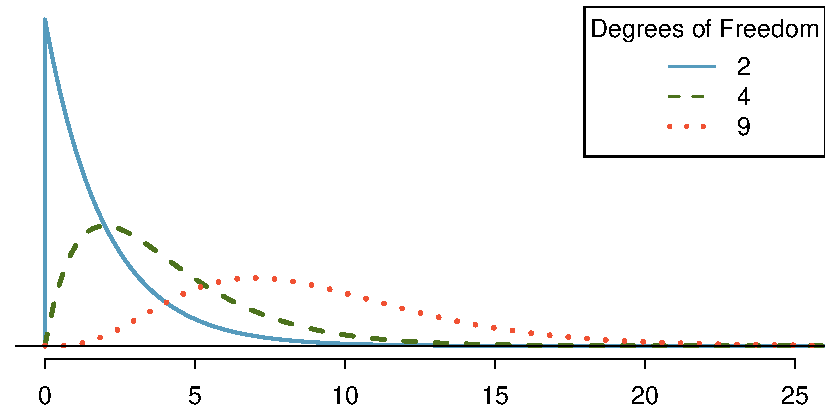
\includegraphics[width=0.9\textwidth]{ch_inference_for_props/figures/chiSquareDistributionWithInceasingDF/chiSquareDistributionWithInceasingDF}
\caption{Three chi-square distributions with varying degrees of freedom.}
\label{chiSquareDistributionWithInceasingDF}
\end{figure}

Figure~\ref{chiSquareDistributionWithInceasingDF} and Guided Practice~\ref{exerChiSquareDistributionDescriptionWithMoreDOF} demonstrate three general properties of chi-square distributions as the degrees of freedom increases: the distribution becomes more symmetric, the center moves to the right, and the variability inflates.

Our principal interest in the chi-square distribution is the calculation of p-values, which (as we have seen before) is related to finding the relevant area in the tail of a distribution. To do so, a new table is needed: the \term{chi-square table}, partially shown in Table~\ref{chiSquareProbabilityTableShort}. A more complete table is presented in Appendix~\vref{chiSquareProbabilityTable}. This table is very similar to the $t$ table from Sections~\ref{oneSampleMeansWithTDistribution} and~\ref{theTDistributionForTheDifferenceOfTwoMeans}: we identify a range for the area, and we examine a particular row for distributions with different degrees of freedom. One important difference from the $t$ table is that the chi-square table only provides upper tail values.

\begin{table}[h]
\centering
\begin{tabular}{r | rrrr | rrrr |}
  \hline
Upper tail & 0.3 & 0.2 & 0.1 & 0.05 & 0.02 & 0.01 & 0.005 & 0.001 \\
  \hline
df \hfill 1 & \footnotesize 1.07 & \footnotesize 1.64 & \footnotesize 2.71 & \footnotesize 3.84 & \footnotesize 5.41 & \footnotesize 6.63 & \footnotesize 7.88 & \footnotesize 10.83 \\
df \hfill 2 & \footnotesize 2.41 & \footnotesize \highlightO{3.22} & \footnotesize \highlightO{4.61} & \footnotesize 5.99 & \footnotesize 7.82 & \footnotesize 9.21 & \footnotesize 10.60 & \footnotesize 13.82 \\
  \em3 & \em\footnotesize 3.66 & \em\footnotesize 4.64 & \em\footnotesize \highlightT{6.25} & \em\footnotesize 7.81 & \em\footnotesize 9.84 & \em\footnotesize 11.34 & \em\footnotesize 12.84 & \em\footnotesize 16.27 \\
  4 & \footnotesize 4.88 & \footnotesize 5.99 & \footnotesize 7.78 & \footnotesize 9.49 & \footnotesize 11.67 & \footnotesize 13.28 & \footnotesize 14.86 & \footnotesize 18.47 \\
  5 & \footnotesize 6.06 & \footnotesize 7.29 & \footnotesize 9.24 & \footnotesize 11.07 & \footnotesize 13.39 & \footnotesize 15.09 & \footnotesize 16.75 & \footnotesize 20.52 \\
  \hline
  6 & \footnotesize 7.23 & \footnotesize 8.56 & \footnotesize 10.64 & \footnotesize 12.59 & \footnotesize 15.03 & \footnotesize 16.81 & \footnotesize 18.55 & \footnotesize 22.46 \\
  7 & \footnotesize 8.38 & \footnotesize 9.80 & \footnotesize 12.02 & \footnotesize 14.07 & \footnotesize 16.62 & \footnotesize 18.48 & \footnotesize 20.28 & \footnotesize 24.32 \\
  \hline
\end{tabular}
\caption{A section of the chi-square table. A complete table is in Appendix~\ref{chiSquareProbabilityTable}.}
\label{chiSquareProbabilityTableShort}
\end{table}

\begin{example}{Figure~\ref{chiSquareAreaAbove6Point25WithDF3} shows a chi-square distribution with 3 degrees of freedom and an upper shaded tail starting at 6.25. Use Table~\ref{chiSquareProbabilityTableShort} to estimate the shaded area.}
This distribution has three degrees of freedom, so only the row with 3 degrees of freedom (df) is relevant. This row has been italicized in the table. Next, we see that the value -- 6.25 -- falls in the column with upper tail area 0.1. That is, the shaded upper tail of Figure~\ref{chiSquareAreaAbove6Point25WithDF3} has area 0.1.
\end{example}

\begin{figure}
\centering
\subfigure[Chi-square with 2 df, area above 4.3 shaded.]{
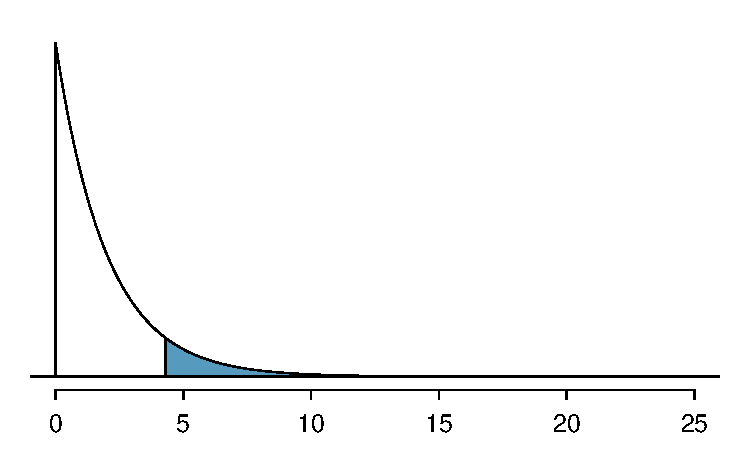
\includegraphics[width=0.475\textwidth]{ch_inference_for_props/figures/arrayOfFigureAreasForChiSquareDistribution/chiSquareAreaAbove4Point3WithDF2/chiSquareAreaAbove4Point3WithDF2}
\label{chiSquareAreaAbove4Point3WithDF2}
}
\subfigure[Chi-square with 3 df, area above 6.25 shaded.]{
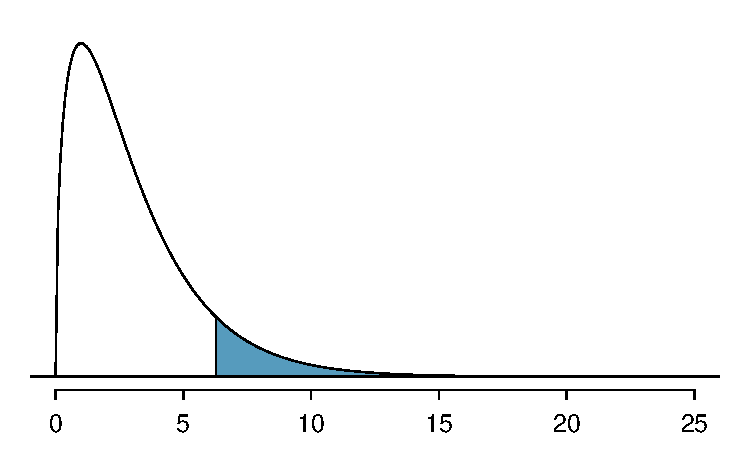
\includegraphics[width=0.475\textwidth]{ch_inference_for_props/figures/arrayOfFigureAreasForChiSquareDistribution/chiSquareAreaAbove6Point25WithDF3/chiSquareAreaAbove6Point25WithDF3}
\label{chiSquareAreaAbove6Point25WithDF3}
}
\subfigure[Chi-square with 3 df, area above 9.21 shaded.]{
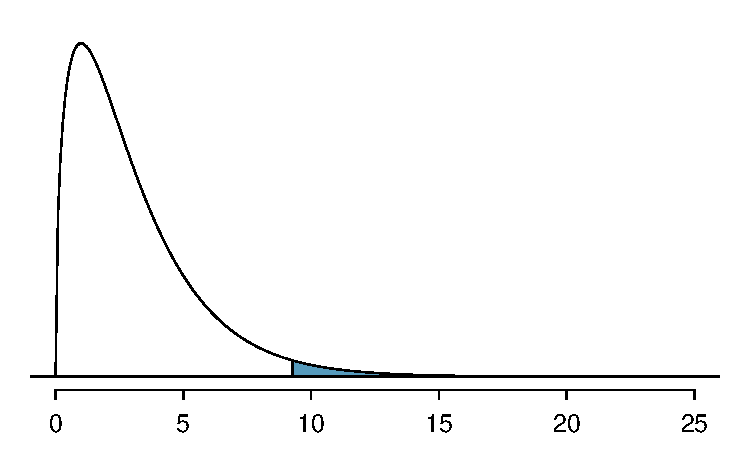
\includegraphics[width=0.475\textwidth]{ch_inference_for_props/figures/arrayOfFigureAreasForChiSquareDistribution/chiSquareAreaAbove9Point21WithDF3/chiSquareAreaAbove9Point21WithDF3}
\label{chiSquareAreaAbove9Point21WithDF3}
}
\subfigure[Chi-square with 4 df, area above 10 shaded.]{
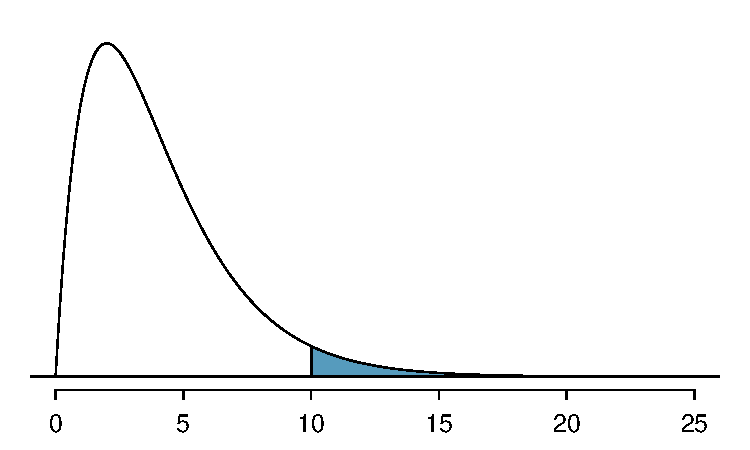
\includegraphics[width=0.475\textwidth]{ch_inference_for_props/figures/arrayOfFigureAreasForChiSquareDistribution/chiSquareAreaAbove10WithDF4/chiSquareAreaAbove10WithDF4}
\label{chiSquareAreaAbove10WithDF4}
}
\subfigure[Chi-square with 5 df, area above 5.1 shaded.]{
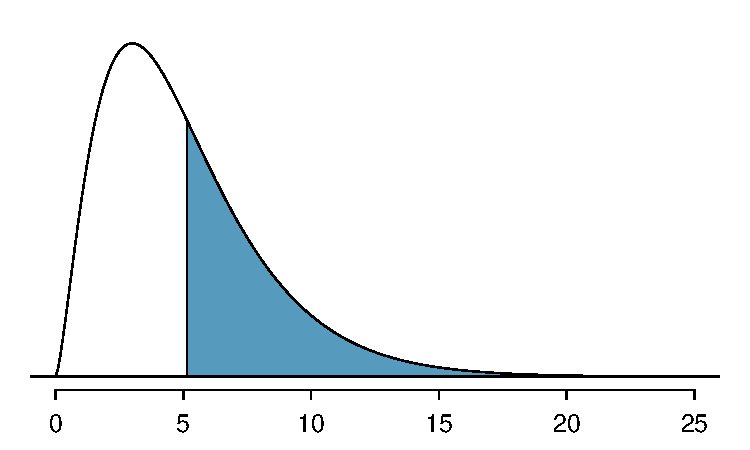
\includegraphics[width=0.475\textwidth]{ch_inference_for_props/figures/arrayOfFigureAreasForChiSquareDistribution/chiSquareAreaAbove5Point1WithDF5/chiSquareAreaAbove5Point1WithDF5}
\label{chiSquareAreaAbove5Point1WithDF5}
}
\subfigure[Chi-square with 7 df, area above 11.7 shaded.]{
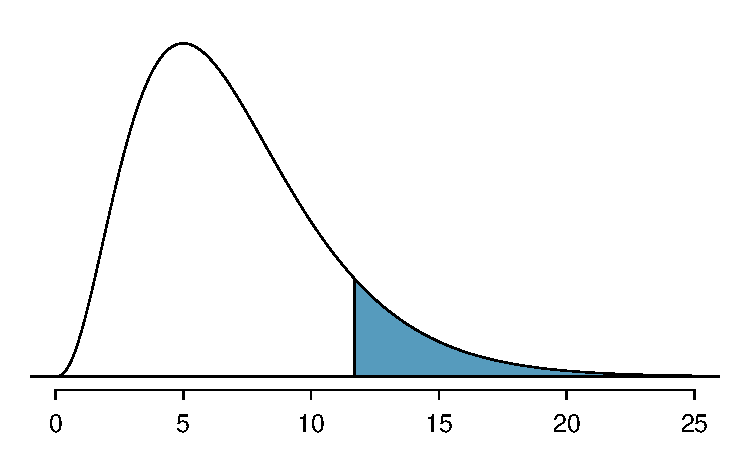
\includegraphics[width=0.475\textwidth]{ch_inference_for_props/figures/arrayOfFigureAreasForChiSquareDistribution/chiSquareAreaAbove11Point7WithDF7/chiSquareAreaAbove11Point7WithDF7}
\label{chiSquareAreaAbove11Point7WithDF7}
}
\caption{\textbf{\subref{chiSquareAreaAbove6Point25WithDF3}} Six chi-square distributions with different right tail areas shaded.}
\label{arrayOfFigureAreasForChiSquareDistribution}
\end{figure}

\begin{example}{We rarely observe the \emph{exact} value in the table. For instance, Figure~\ref{chiSquareAreaAbove4Point3WithDF2} shows the upper tail of a chi-square distribution with 2 degrees of freedom. The lower bound for this upper tail is at 4.3, which does not fall in Table~\ref{chiSquareProbabilityTableShort}. Find the approximate tail area.}
The cutoff 4.3 falls between the second and third columns in the 2 degrees of freedom row. Because these columns correspond to tail areas of 0.2 and 0.1, we can be certain that the area shaded in Figure~\ref{chiSquareAreaAbove4Point3WithDF2} is between 0.1 and 0.2.
\end{example}

Using a calculator or statistical software allows us to get more precise areas under the chi-square curve than we can get from the table alone.

\begin{termBox}{\tBoxTitle{TI Calculator: finding areas under the chi-square curve}
Use the \textbf{$X^2$cdf} command to find areas under the chi-square curve.
\begin{enumerate}
\setlength{\itemsep}{0mm}
\item Hit 2ND VARS (i.e. DISTR).
\item Choose 8: $X^2$cdf.
\item Enter the lower bound (generally the chi-square value).
\item Enter the upper bound (use a large number, such as 1000).
\item Enter the degrees of freedom.
\item Choose Paste and hit ENTER.
\begin{itemize}
\item[TI-83: ] Do steps 1 - 2, then type the lower bound, upper bound, and degrees of freedom separated by commas. e.g. $X^2$cdf(5, 1000, 3), and hit ENTER.
\end{itemize}
\end{enumerate}
}
\end{termBox}

\begin{exercise}
Figure~\ref{chiSquareAreaAbove5Point1WithDF5} shows an upper tail for a chi-square distribution with 5 degrees of freedom and a cutoff of 5.1. Find the tail area using a calculator.\footnote{Using $X^2$cdf(5.1, 1000, 5) gives 0.4038.}
\end{exercise}

\begin{exercise}
Figure~\ref{chiSquareAreaAbove11Point7WithDF7} shows a cutoff of 11.7 on a chi-square distribution with 7 degrees of freedom. Find the area of the upper tail.\footnote{The area is 0.1109.}
\end{exercise}

\begin{exercise}
Figure~\ref{chiSquareAreaAbove10WithDF4} shows a cutoff of 10 on a chi-square distribution with 4 degrees of freedom. Find the area of the upper tail.\footnote{The area is 0.4043.}
\end{exercise}

\begin{exercise}
Figure~\ref{chiSquareAreaAbove9Point21WithDF3} shows a cutoff of 9.21 with a chi-square distribution with 3 df. Find the area of the upper tail.\footnote{The area is 0.0266.}
\end{exercise}


\subsection{Finding a p-value for a chi-square distribution}
\label{pValueForAChiSquareTest}

\index{data!racial make-up of jury|(}
In Section~\ref{chiSquareTestStatistic}, we identified a new test statistic ($X^2$) within the context of assessing whether there was evidence of racial bias in how jurors were sampled. The null hypothesis represented the claim that jurors were randomly sampled and there was no racial bias. The alternative hypothesis was that there was racial bias in how the jurors were sampled.

We determined that a large $X^2$ value would suggest strong evidence favoring the alternative hypothesis: that there was racial bias. However, we could not quantify what the chance was of observing such a large test statistic ($X^2=5.89$) if the null hypothesis actually was true. This is where the chi-square distribution becomes useful. If the null hypothesis was true and there was no racial bias, then $X^2$ would follow a chi-square distribution, with three degrees of freedom in this case. Under certain conditions, the statistic $X^2$ follows a chi-square distribution with $k-1$ degrees of freedom, where $k$ is the number of bins or categories of the variable.

\begin{example}{How many categories were there in the juror example? How many degrees of freedom should be associated with the chi-square distribution used for $X^2$?}
In the jurors example, there were $k=4$ categories: white, black, Hispanic, and other. According to the rule above, the test statistic $X^2$ should then follow a chi-square distribution with $k-1 = 3$ degrees of freedom if $H_0$ is true.
\end{example}

Just like we checked sample size conditions to use the normal model in earlier sections, we must also check a sample size condition to safely apply the chi-square distribution for $X^2$. Each expected count must be at least 5. In the juror example, the expected counts were 198, 19.25, 33, and 24.75, all easily above~5, so we can apply the chi-square model to the test statistic, $X^2=5.89$.

\begin{example}{If the null hypothesis is true, the test statistic $X^2=5.89$ would be closely associated with a chi-square distribution with three degrees of freedom. Using this distribution and test statistic, identify the p-value and state whether or not there is evidence of racial bias in the juror selection.}
The chi-square distribution and p-value are shown in Figure~\ref{jurorHTPValueShown}. Because larger chi-square values correspond to stronger evidence against the null hypothesis, we shade the upper tail to represent the p-value. Using the chi-square table in Appendix~\ref{chiSquareProbabilityTable} or the short table on page~\pageref{chiSquareProbabilityTableShort}, we can determine that the area is between 0.1 and 0.2. That is, the p-value is larger than 0.1 but smaller than 0.2. Generally we do not reject the null hypothesis with such a large p-value. In other words, the data do not provide convincing evidence of racial bias in the juror selection.
\index{data!racial make-up of jury|)}
\end{example}

\begin{figure}[h]
\centering
\includegraphics[width=0.61\textwidth]{ch_inference_for_props/figures/jurorHTPValueShown/jurorHTPValueShown}
\caption{The p-value for the juror hypothesis test is shaded in the chi-square distribution with $df=3$.}
\label{jurorHTPValueShown}
\end{figure}

The test that we just carried out regarding jury selection is known as the \term{$X^2$ goodness of fit test}. It is called ``goodness of fit" because we test whether or not the proposed or expected distribution is a good fit for the observed data.

\begin{termBox}{\tBoxTitle{Chi-square goodness of fit test for one-way table}
Suppose we are to evaluate whether there is convincing evidence that a set of observed counts $O_1$, $O_2$, ..., $O_k$ in $k$ categories are unusually different from what might be expected under a null hypothesis. Call the \emph{expected counts} that are based on the null hypothesis $E_1$, $E_2$, ..., $E_k$. If each expected count is at least 5 and the null hypothesis is true, then the test statistic below follows a chi-square distribution with $k-1$ degrees of freedom:
\begin{align*}
X^2 = \frac{(O_1 - E_1)^2}{E_1} + \frac{(O_2 - E_2)^2}{E_2} + \cdots + \frac{(O_k - E_k)^2}{E_k}
\end{align*}
The p-value for this test statistic is found by looking at the upper tail of this chi-square distribution. We consider the upper tail because larger values of $X^2$ would provide greater evidence against the null hypothesis.}
\end{termBox}

\begin{tipBox}{\tipBoxTitle{Conditions for the chi-square goodness of fit test}
There are two conditions that must be checked before performing a chi-square goodness of fit test. If these conditions are not met, this test should not be used.\vspace{-1mm}
\begin{description}
\setlength{\itemsep}{0mm}
\item[Simple random sample.] The data must be arrived at by taking a simple random sample from the population of interest. The observed counts can then be organized into a list or one-way table.
\item[All Expected Counts at least 5] Each particular scenario (i.e. cell count) must have at least 5~expected cases.
\vspace{-2mm}
\end{description}
}
\end{tipBox}

%\Add{
%\begin{example}{Comment on the appropriateness of the $X^2$ goodness of fit test for the following data.
%\begin{center}
%\begin{tabular}{l c c}
%\hline
%Outcome of coin toss & Head & Tail \\
%\hline
%Observed counts & 56 & 44 \\
%Expected counts & 50 & 50 \\
%\hline
%\end{tabular}
%\end{center}}
%While it would be possible to carry out the $X^2$ goodness of fit test, it would make more sense to do a 1-proportion Z test with H$_0: p=0.5$ and $\hat{p}=56/100$.
%\end{example}
%}


\subsection{Evaluating goodness of fit for a distribution}

\begin{termBox}{\tBoxTitle[]{Goodness of fit test for a one-way table}
\begin{enumerate}
\setlength{\itemsep}{0mm}
\item State the name of the test being used: $X^2$ goodness of fit test.
\item Verify conditions.\vspace{-1.5mm}
\begin{itemize}
\setlength{\itemsep}{0mm}
\item a random sample
\item all expected counts $\ge 5$ (calculate and record expected counts)
\end{itemize}
\item Write the hypotheses in plain language. No mathematical notation is needed for this test.\vspace{-1.5mm}
\begin{itemize}
\setlength{\itemsep}{0mm}
\item H$_0$: The distribution of [...] matches [the expected distribution].
\item H$_A$: The distribution of [....] does not match [the expected distribution]
\end{itemize}
\item Identify the significance level $\alpha$.
\item Calculate the test statistic and degrees of freedom.\vspace{-2mm}
\begin{align*}
X^2 &= \sum{\frac{\text{(observed counts - expected counts)}^2}{\text{expected counts}}} \\
df &= (\# \text{ of categories} - 1)
\end{align*}
\item Find the p-value and compare it to $\alpha$ to determine whether to reject or not reject $H_0$.
\item Write the conclusion in the context of the question.
\end{enumerate}}
\end{termBox}

%\Comment{I propose removing this who section/example in favor of a simpler example}
Section~\ref{geomDist} would be useful background reading for this example, but it is not a prerequisite.

\index{data!S\&P500 stock data|(}

We can apply our new chi-square testing framework to the second problem in this section: evaluating whether a certain statistical model fits a data set. Daily stock returns from the S\&P500 for 1990-2011 can be used to assess whether stock activity each day is independent of the stock's behavior on previous days. This sounds like a very complex question, and it is, but a chi-square test can be used to study the problem. We will label each day as \resp{Up} or \resp{Down} (\resp{D}) depending on whether the market was up or down that day. For example, consider the following changes in price, their new labels of up and down, and then the number of days that must be observed before each \resp{Up} day:
\begin{center}\footnotesize
\begin{tabular}{lc ccc ccc ccc cc}
Change in price		&\hspace{-1mm}	& \footnotesize2.52 &
	\footnotesize-1.46 & \footnotesize 0.51 &
	\footnotesize-4.07 & \footnotesize3.36 &
	\footnotesize1.10 &
	\footnotesize-5.46 & \footnotesize-1.03 & \footnotesize-2.99 & \footnotesize1.71 \\
Outcome	 & \hspace{-1mm} &
	Up &
	D & Up &
	D & Up &
	Up &
	D & D & D & Up \\
\footnotesize Days to Up & \hspace{-1mm} & 1 & - & 2 & - & 2 & 1 & - & - & - & 4 \\
\end{tabular}
\end{center}
If the days really are independent, then the number of days until a positive trading day should follow a geometric distribution. The geometric distribution describes the probability of waiting for the $k^{th}$ trial to observe the first success. Here each up day (Up) represents a success, and down (D) days represent failures. In the data above, it took only one day until the market was up, so the first wait time was 1 day. It took two more days before we observed our next \resp{Up} trading day, and two more for the third \resp{Up} day. We would like to determine if these counts (1, 2, 2, 1, 4, and so on) follow the geometric distribution. Table~\ref{sAndP500For1990To2011TimeToPosTrade} shows the number of waiting days for a positive trading day during 1990-2011 for the S\&P500.

\begin{table}[h]
\centering
\begin{tabular}{ll ccc ccc c ll}
\hline
Days	 & \hspace{2mm} & 1 & 2 & 3 & 4 & 5 & 6 & 7+ & \hspace{2mm} & Total \\
Observed &		& 1532 & 760 & 338 & 194 & 74 & 33 & 17 & & 2948 \\
\hline
\end{tabular}
\caption{Observed distribution of the waiting time until a positive trading day for the S\&P500, 1990-2011.}
\label{sAndP500For1990To2011TimeToPosTrade}
\end{table}

We consider how many days one must wait until observing an \resp{Up} day on the S\&P500 stock exchange. If the stock activity was independent from one day to the next and the probability of a positive trading day was constant, then we would expect this waiting time to follow a \emph{geometric distribution}. We can organize this into a hypothesis framework:
\begin{itemize}
\item[$H_0$:] The stock market being up or down on a given day is independent from all other days. We will consider the number of days that pass until an \resp{Up} day is observed. Under this hypothesis, the number of days until an \resp{Up} day should follow a geometric distribution.
\item[$H_A$:] The stock market being up or down on a given day is not independent from all other days. Since we know the number of days until an \resp{Up} day would follow a geometric distribution under the null, we look for deviations from the geometric distribution, which would support the alternative hypothesis.
\end{itemize}
There are important implications in our result for stock traders: if information from past trading days is useful in telling what will happen today, that information may provide an advantage over other traders.

We consider data for the S\&P500 from 1990 to 2011 and summarize the waiting times in Table~\ref{sAndP500For1990To2011TimeToPosTrade2} and Figure~\ref{geomFitEvaluationForSP500For1990To2011}. The S\&P500 was positive on 53.2\% of those days.

\begin{table}
\centering
\begin{tabular}{ll ccc ccc c ll}
\hline
Days	 & \hspace{1mm} & 1 & 2 & 3 & 4 & 5 & 6 & 7+ & \hspace{1mm} & Total \\
\hline
Observed &		& 1532 & 760 & 338 & 194 & 74 & 33 & 17 & & 2948 \\
Geometric Model &		& 1569 & 734 & 343 & 161 & 75 & 35 & 31 & & 2948 \\
\hline
\end{tabular}
\caption{Distribution of the waiting time until a positive trading day. The expected counts based on the geometric model are shown in the last row. To find each expected count, we identify the probability of waiting $D$ days based on the geometric model ($P(D) = (1-0.532)^{D-1}(0.532)$) and multiply by the total number of streaks, 2948. For example, waiting for three days occurs under the geometric model about $0.468^2\times 0.532 = 11.65\%$ of the time, which corresponds to $0.1165\times 2948 = 343$ streaks.}
\label{sAndP500For1990To2011TimeToPosTrade2}
\end{table}

\begin{figure}
\centering
\includegraphics[width=0.98\textwidth]{ch_inference_for_props/figures/geomFitEvaluationForSP500For1990To2011/geomFitEvaluationForSP500For1990To2011}
\caption{Side-by-side bar plot of the observed and expected counts for each waiting time.}
\label{geomFitEvaluationForSP500For1990To2011}
\end{figure}

Because applying the chi-square framework requires expected counts to be at least~5, we have \emph{binned} together all the cases where the waiting time was at least 7 days to ensure each expected count is well above this minimum. The actual data, shown in the \emph{Observed} row in Table~\ref{sAndP500For1990To2011TimeToPosTrade2}, can be compared to the expected counts from the \emph{Geometric Model} row. The method for computing expected counts is discussed in Table~\ref{sAndP500For1990To2011TimeToPosTrade2}. In general, the expected counts are determined by (1) identifying the null proportion associated with each bin, then (2) multiplying each null proportion by the total count to obtain the expected counts. That is, this strategy identifies what proportion of the total count we would expect to be in each bin.

\begin{example}{Do you notice any unusually large deviations in the graph? Can you tell if these deviations are due to chance just by looking?}
It is not obvious whether differences in the observed counts and the expected counts from the geometric distribution are significantly different. That is, it is not clear whether these deviations might be due to chance or whether they are so strong that the data provide convincing evidence against the null hypothesis. However, we can perform a chi-square test using the counts in Table~\ref{sAndP500For1990To2011TimeToPosTrade2}.
\end{example}

\begin{exercise}
Table~\ref{sAndP500For1990To2011TimeToPosTrade2} provides a set of count data for waiting times ($O_1=1532$, $O_2=760$, ...) and expected counts under the geometric distribution ($E_1=1569$, $E_2=734$, ...). Compute the chi-square test statistic, $X^2$.\footnote{$X^2=\frac{(1532-1569)^2}{1569} + \frac{(760-734)^2}{734} + \cdots + \frac{(17-31)^2}{31} = 15.08$}
\end{exercise}

\begin{exercise}
Because the expected counts are all at least~5, we can safely apply the chi-square distribution to $X^2$. However, how many degrees of freedom should we~use?\footnote{There are $k=7$ groups, so we use $df=k-1=6$.}
\end{exercise}

\begin{example}{If the observed counts follow the geometric model, then the chi-square test statistic $X^2=15.08$ would closely follow a chi-square distribution with $df=6$. Using this information, compute a p-value.} \label{RejectGeomModelForSP500StockDataFor1990To2011}
Figure~\ref{geomFitPValueForSP500For1990To2011} shows the chi-square distribution, cutoff, and the shaded p-value. If we look up the statistic $X^2=15.08$ in Appendix~\ref{chiSquareProbabilityTable}, we find that the p-value is between 0.01 and 0.02. In other words, we have sufficient evidence to reject the notion that the wait times follow a geometric distribution, i.e. trading days are not independent and past days may help predict what the stock market will do today.
\end{example}

\begin{figure}
\centering
\includegraphics[width=0.9\textwidth]{ch_inference_for_props/figures/geomFitPValueForSP500For1990To2011/geomFitPValueForSP500For1990To2011}
\caption{Chi-square distribution with 6 degrees of freedom. The p-value for the stock analysis is shaded.}
\label{geomFitPValueForSP500For1990To2011}
\end{figure}

\begin{example}{In Example~\ref{RejectGeomModelForSP500StockDataFor1990To2011}, we rejected the null hypothesis that the trading days are independent. Why is this so important?}
Because the data provided strong evidence that the geometric distribution is not appropriate, we reject the claim that trading days are independent. While it is not obvious how to exploit this information, it suggests there are some hidden patterns in the data that could be interesting and possibly useful to a stock trader.
\index{data!S\&P500 stock data|)}
\end{example}

\subsection{Calculator: chi-square goodness of fit test\vspace{-3mm}}

\begin{termBox}{\tBoxTitle{TI calculator: Carrying out the chi-square goodness of fit test\vspace{0.5mm}}
Use \textbf{STAT, TESTS, $X^2$GOF-Test}.
\begin{enumerate}
\setlength{\itemsep}{0mm}
\item Enter the observed counts into list L1 and the expected counts into list L2.
\item Choose STAT.
\item Right arrow to TESTS.
\item Down arrow and choose D: $X^2$GOF-Test.
\item Leave Observed: L1 and Expected: L2.
\item Enter the degrees of freedom after df:
\item Choose Calculate and hit ENTER, which returns: \\
\begin{tabular}{l ll}
\hspace{3mm}&
	$X^2$
	&\quad chi-square value \\
&
	\text{p}
	&\quad p-value \\
&
	df
	&\quad  degrees of freedom
\end{tabular}
\begin{itemize}
\item[TI-83: ] Unfortunately the TI-83 does not have this test built in. To carry out the test manually, make list L3 = (L1 - L2)$^2$ / L2 and do 1-Var-Stats on L3. The sum of L3 will correspond to the value of $X^2$ for this test.
\end{itemize}
\end{enumerate}
}
\end{termBox}

\begin{table}[h]
\centering
\begin{tabular}{ll ccc ccc c ll}
\hline
Days	 & \hspace{1mm} & 1 & 2 & 3 & 4 & 5 & 6 & 7+ & \hspace{1mm} & Total \\
\hline
Observed &		& 1532 & 760 & 338 & 194 & 74 & 33 & 17 & & 2948 \\
Geometric Model &  & 1569 & 734 & 343 & 161 & 75 & 35 & 31 & & 2948 \\
\hline
\end{tabular}
\caption{Distribution of the waiting time until a positive trading day. The expected counts based on the geometric model are shown in the last row. }
\end{table}

\begin{exercise}
Use the data above and a calculator to find the $X^2$ statistic, df, and p-value for chi-square goodness of fit test.\footnote{First enter the observed values into L1 and the expected values into L2. Use STAT, TESTS, $X^2$GOF-Test. $X^2=15.08$, $df=6$, p-value$=0.0196$.}
\end{exercise}



%__________________
\section{Homogeneity and independence in two-way tables}
\label{twoWayTablesAndChiSquare}

\index{data!search algorithm|(}

Google is constantly running experiments to test new search algorithms. For example, Google might test three algorithms using a sample of 10,000 google.com search queries. Table~\ref{googleSearchAlgorithmByAlgorithmOnly} shows an example of 10,000 queries split into three algorithm groups.\footnote{Google regularly runs experiments in this manner to help improve their search engine. It is entirely possible that if you perform a search and so does your friend, that you will have different search results. While the data presented in this section resemble what might be encountered in a real experiment, these data are simulated.} The group sizes were specified before the start of the experiment to be 5000 for the current algorithm and 2500 for each test algorithm.

\begin{table}[h]
\centering
\begin{tabular}{ll ccc ll}
\hline
Search algorithm	 & \hspace{1mm} & current & test 1 & test 2 & \hspace{1mm} & Total \\
Counts &		& 5000 & 2500 & 2500 & & 10000 \\
\hline
\end{tabular}
\caption{Google experiment breakdown of test subjects into three search groups.}
\label{googleSearchAlgorithmByAlgorithmOnly}
\end{table}


\begin{example}{What is the ultimate goal of the Google experiment? What are the null and alternative hypotheses, in regular words?}
The ultimate goal is to see whether there is a difference in the performance of the algorithms. The hypotheses can be described as the following:
\begin{itemize}
\item[$H_0$:] The algorithms each perform equally well.
\item[$H_A$:] The algorithms do not perform equally well.
\end{itemize}
\end{example}
%\Comment{exports from here to calculator section on two-way tables}

In this experiment, the explanatory variable is the search algorithm. However, an outcome variable is also needed. This outcome variable should somehow reflect whether the search results align with the user's interests. One possible way to quantify this is to determine whether (1)~there was no new, related search, and the user clicked one of the links provided, or (2)~there was a new, related search performed by the user. Under scenario~(1), we might think that the user was satisfied with the search results. Under scenario~(2), the search results probably were not relevant, so the user tried a second search.

Table~\ref{googleSearchAlgorithmByAlgorithmAndPerformanceWithTotals} provides the results from the experiment. These data are very similar to the count data in Section~\ref{oneWayChiSquare}. However, now the different combinations of two variables are binned in a \emph{two-way} table. In examining these data, we want to evaluate whether there is strong evidence that at least one algorithm is performing better than the others. To do so, we apply a chi-square test to this two-way table. The ideas of this test are similar to those ideas in the one-way table case. However, degrees of freedom and expected counts are computed a little differently than before.

\begin{table}[h]
\centering
\quad \quad \quad \quad Search algorithm \\
\begin{tabular}{ll ccc ll}
\hline
 & \hspace{1mm} & current & test 1 & test 2 & \hspace{1mm} & Total \\
\hline
No new search				   & & 3511    & 1749 & 1818 & 				& 7078 \\
New search				   & & 1489    & 751	& 682    &				& 2922 \\
\hline
Total						   & & 5000    & 2500 & 2500 & 				& 10000 \\
\hline
\end{tabular}
\caption{Results of the Google search algorithm experiment.}
\label{googleSearchAlgorithmByAlgorithmAndPerformanceWithTotals}
\end{table}

\begin{tipBox}{\tipBoxTitle{What is so different about one-way tables and two-way tables?}
A one-way table describes counts for each outcome in a single variable. A two-way table describes counts for \emph{combinations} of outcomes for two variables. When we consider a two-way table, we often would like to know, are these variables related in any way?}
\end{tipBox}

The hypothesis test for this Google experiment is really about assessing whether there is statistically significant evidence that the choice of the algorithm affects whether a user performs a second search. In other words, the goal is to check whether the the three search algorithms perform differently.


\subsection{Expected counts in two-way tables}

\begin{example}{From the experiment, we estimate the proportion of users who were satisfied with their initial search (no new search) as $7078/10000 = 0.7078$. If there really is no difference among the algorithms and 70.78\% of people are satisfied with the search results, how many of the 5000 people in the ``current algorithm'' group would be expected to not perform a new search?} \label{googleExampleComputingTheExpectedNumberOfCurrentGroupWithNoNewSearch}
About 70.78\% of the 5000 would be satisfied with the initial search:
$$ 0.7078\times 5000 = 3539\text{ users} $$
That is, if there was no difference between the three groups, then we would expect 3539 of the current algorithm users not to perform a new search.
\end{example}

\begin{exercise}\label{googleExampleComputingTheExpectedNumberOfNewAlgGroupWithNoNewSearch}
Using the same rationale described in Example~\ref{googleExampleComputingTheExpectedNumberOfCurrentGroupWithNoNewSearch}, about how many users in each test group would not perform a new search if the algorithms were equally helpful?\footnote{We would expect $0.7078*2500 = 1769.5$. It is okay that this is a fraction.}
\end{exercise}

We can compute the expected number of users who would perform a new search for each group using the same strategy employed in Example~\ref{googleExampleComputingTheExpectedNumberOfCurrentGroupWithNoNewSearch} and Guided Practice~\ref{googleExampleComputingTheExpectedNumberOfNewAlgGroupWithNoNewSearch}. These expected counts were used to construct Table~\ref{googleSearchAlgorithmByAlgorithmAndPerformanceWithExpectedCounts}, which is the same as Table~\ref{googleSearchAlgorithmByAlgorithmAndPerformanceWithTotals}, except now the expected counts have been added in parentheses.

\begin{table}[h]
\centering
\begin{tabular}{l lll lll lll l}
\hline
Search algorithm\hspace{2mm} & \multicolumn{2}{l}{current} &&
					\multicolumn{2}{l}{test 1} &&
					\multicolumn{2}{l}{test 2} & \hspace{0mm} & Total \\
\hline
No new search		   & 3511 &\highlightO{\footnotesize(3539)}    &&
					1749 &\highlightO{\footnotesize(1769.5)}	&&
					1818 &\highlightO{\footnotesize(1769.5)} &	& 7078 \\
New search		   & 1489 &\highlightO{\footnotesize(1461)}    &&
					751 &\highlightO{\footnotesize(730.5)}	&&
					682 &\highlightO{\footnotesize(730.5)}    &		& 2922 \\
\hline
Total				   & 5000 &&& 	2500 &&& 	2500 &&& 	10000 \\
\hline
\end{tabular}
\caption{The observed counts and the \highlightO{(expected counts)}.}
\label{googleSearchAlgorithmByAlgorithmAndPerformanceWithExpectedCounts}
\end{table}

The examples and exercises above provided some help in computing expected counts. In general, expected counts for a two-way table may be computed using the row totals, column totals, and the table total. For instance, if there was no difference between the groups, then about 70.78\% of each column should be in the first row:
\begin{align*}
0.7078\times (\text{column 1 total}) &= 3539 \\
0.7078\times (\text{column 2 total}) &= 1769.5 \\
0.7078\times (\text{column 3 total}) &= 1769.5
\end{align*}
Looking back to how the fraction 0.7078 was computed -- as the fraction of users who did not perform a new search ($7078/10000$) -- these three expected counts could have been computed as
\begin{align*}
\left(\frac{\text{row 1 total}}{\text{table total}}\right)\text{(column 1 total)} &= 3539 \\
\left(\frac{\text{row 1 total}}{\text{table total}}\right)\text{(column 2 total)} &= 1769.5 \\
\left(\frac{\text{row 1 total}}{\text{table total}}\right)\text{(column 3 total)} &= 1769.5
\end{align*}
This leads us to a general formula for computing expected counts in a two-way table when we would like to test whether there is strong evidence of an association between the column variable and row variable.

\begin{termBox}{\tBoxTitle{Computing expected counts in a two-way table}
To identify the expected count for the $i^{th}$ row and $j^{th}$ column, compute
$$\text{Expected Count}_{\text{row }i,\text{ col }j} = \frac{(\text{row $i$ total}) \times  (\text{column $j$ total})}{\text{table total}}\vspace{2mm}$$}
\end{termBox}


\subsection{The chi-square test of homogeneity for two-way tables}

The chi-square test statistic for a two-way table is found the same way it is found for a one-way table. For each table count, compute
\begin{align*}
&\text{General formula}& &\frac{(\text{observed count } - \text{ expected count})^2}{\text{expected count}} \\
&\text{Row 1, Col 1}& &\frac{(3511 - 3539)^2}{3539} = 0.222 \\
&\text{Row 1, Col 2}& &\frac{(1749 - 1769.5)^2}{1769.5} = 0.237 \\
& \hspace{9mm}\vdots & &\hspace{13mm}\vdots \\
&\text{Row 2, Col 3}& &\frac{(682 - 730.5)^2}{730.5} = 3.220
\end{align*}
Adding the computed value for each cell gives the chi-square test statistic $X^2$:
$$X^2 = 0.222 + 0.237 + \dots + 3.220 = 6.120$$
Just like before, this test statistic follows a chi-square distribution. However, the degrees of freedom are computed a little differently for a two-way table.\footnote{Recall: in the one-way table, the degrees of freedom was the number of cells minus 1.} For two way tables, the degrees of freedom is equal to
\begin{align*}
df = \text{(number of rows - 1)}\times \text{(number of columns - 1)}
\end{align*}
In our example, the degrees of freedom parameter is
\begin{align*}
df = (2-1)\times (3-1) = 2
\end{align*}
If the null hypothesis is true (i.e. the algorithms are equally useful), then the test statistic $X^2 = 6.12$ closely follows a chi-square distribution with 2 degrees of freedom. Using this information, we can compute the p-value for the test, which is depicted in Figure~\ref{googleHTForDiffAlgPerformancePValue}.

\begin{termBox}{\tBoxTitle{Computing degrees of freedom for a two-way table}
When applying the chi-square test to a two-way table, we use
$$ df = (R-1)\times (C-1) $$
where $R$ is the number of rows in the table and $C$ is the number of columns.}
\end{termBox}

\begin{tipBox}{\tipBoxTitle{Use two-proportion methods for 2-by-2 contingency tables}
When analyzing 2-by-2 contingency tables, use the two-proportion methods introduced in Section~\ref{differenceOfTwoProportions}.}
\end{tipBox}

\begin{figure}[h]
\centering
\includegraphics[width=0.7\textwidth]{ch_inference_for_props/figures/googleHTForDiffAlgPerformancePValue/googleHTForDiffAlgPerformancePValue}
\caption{Computing the p-value for the Google hypothesis test.}
\label{googleHTForDiffAlgPerformancePValue}
\end{figure}

\begin{tipBox}{\tipBoxTitle{Conditions for the chi-square test of homeneity}
There are two conditions that must be checked before performing a chi-square test of homogeneity. If these conditions are not met, this test should not be used.\vspace{-1mm}
\begin{description}
\setlength{\itemsep}{0mm}
\item[Mutliple random samples or randomly allocated treatments. ]Data collected by multiple independent random samples or multiple randomlly allocated treatments. Data can then be organized into a two-way table.
\item[All Expected Counts at least 5. ] All of the expected counts must be at least~5.
\vspace{-1mm}
\end{description}}
\end{tipBox}

\begin{example}{Compute the p-value and draw a conclusion about whether the search algorithms have different performances.}
Looking in Appendix~\ref{chiSquareProbabilityTable} on page~\pageref{chiSquareProbabilityTable}, we examine the row corresponding to 2 degrees of freedom. The test statistic, $X^2=6.120$, falls between the fourth and fifth columns, which means the p-value is between 0.02 and 0.05. Because we typically test at a significance level of $\alpha=0.05$ and the p-value is less than 0.05, the null hypothesis is rejected. That is, the data provide convincing evidence that there is some difference in performance among the algorithms.
\index{data!search algorithm|)}
\end{example}

%	Approve	Disapprove
%Obama	56	41
%Dem	49	43
%Rep	36	56
%http://www.people-press.org/2012/03/14/romney-leads-gop-contest-trails-in-matchup-with-obama/
%March 7-11, 2012
%1503 adults


\subsection{The chi-square test of independence for two-way tables}

The chi-square test of Independence proceeds exactly like the chi-square test of homogeneity, except that it applies when there is only one random sample (versus multiple random samples or an experiment with multiple randomly allocated treatments). The null claim is always that two variables are independent, while the alternate claim is that the variables are dependent.

\begin{example}{\index{data!approval ratings|(}Table~\ref{pewResearchPollOnApprovalRatingsForChiSquareSectionExampleAndExercises} summarizes the results of a Pew Research poll.\footnote{See the Pew Research website: {\scriptsize\href{http://www.people-press.org/2012/03/14/romney-leads-gop-contest-trails-in-matchup-with-obama/}{www.people-press.org/2012/03/14/romney-leads-gop-contest-trails-in-matchup-with-obama}}. The counts in Table~\ref{pewResearchPollOnApprovalRatingsForChiSquareSectionExampleAndExercises} are approximate.} We would like to determine if three groups and approval ratings are associated. What are appropriate hypotheses for such a test?}\label{hypothesisTestSetupForPewResearchPollOnApprovalRatingsForChiSquareSection}
\begin{itemize}
\item[$H_0$:] The ratings are independent of the group. (There is no difference in approval ratings between the three groups.)
\item[$H_A$:] The ratings are dependent on the group. (There is some difference in approval ratings between the three groups, e.g. perhaps Obama's approval differs from Democrats in Congress.)
\end{itemize}
\end{example}

\begin{table}
\centering
\begin{tabular}{ll ccc ll}
& & & \multicolumn{2}{c}{Congress} & \\
\cline{4-5}
 & \hspace{1mm} & Obama & Democrats & Republicans & \hspace{1mm} & Total \\
\hline
Approve				   & & 842    & 736 & 541   & 				& 2119 \\
Disapprove			   & & 616    & 646 & 842   &				& 2104 \\
\hline
Total					   & & 1458    & 1382 & 1383 & 				& 4223 \\
\hline
\end{tabular}
\caption{Pew Research poll results of a March 2012 poll.}
\label{pewResearchPollOnApprovalRatingsForChiSquareSectionExampleAndExercises}
\end{table}

\begin{exercise}
A chi-square test for a two-way table may be used to test the hypotheses in Example~\ref{hypothesisTestSetupForPewResearchPollOnApprovalRatingsForChiSquareSection}. As a first step, compute the expected values for each of the six table cells.\footnote{The expected count for row one / column one is found by multiplying the row one total (2119) and column one total (1458), then dividing by the table total (4223): $\frac{2119\times 1458}{3902} = 731.6$. Similarly for the first column and the second row: $\frac{2104\times 1458}{4223} = 726.4$. Column 2: 693.5 and 688.5. Column 3: 694.0 and 689.0}
% R <- c(2119, 2104); C <- c(1458, 1382, 1383); R*C[1]/sum(C); R*C[2]/sum(C); R*C[3]/sum(C)
\end{exercise}

\begin{exercise}
Compute the chi-square test statistic.\footnote{For each cell, compute $\frac{(\text{obs} - \text{exp})^2}{exp}$. For instance, the first row and first column: $\frac{(842-731.6)^2}{731.6} = 16.7$. Adding the results of each cell gives the chi-square test statistic: {\scriptsize$X^2 = 16.7 + \cdots + 34.0 = 106.4$}.}
%R <- c(2119, 2104); C <- c(1458, 1382, 1383); CC <- c(842, 616, 736, 646, 541, 842); EE <- round(c(R*C[1]/sum(C), R*C[2]/sum(C), R*C[3]/sum(C)), 1); (CC-EE)^2/EE; sum((CC-EE)^2/EE)
\end{exercise}

\begin{exercise}
Because there are 2 rows and 3 columns, the degrees of freedom for the test is $df=(2-1)\times (3-1) = 2$. Use $X^2=106.4$, $df=2$, and the chi-square table on page~\pageref{chiSquareProbabilityTable} to evaluate whether to reject the null hypothesis.\footnote{The test statistic is larger than the right-most column of the $df=2$ row of the chi-square table, meaning the p-value is less than 0.001. That is, we reject the null hypothesis because the p-value is less than 0.05, and we conclude that Americans' approval has differences among Democrats in Congress, Republicans in Congress, and the president.}
\end{exercise}
\index{data!approval ratings|)}

\begin{tipBox}{\tipBoxTitle{Conditions for the chi-square test of independence}
There are two conditions that must be checked before performing a chi-square test of independence. If these conditions are not met, this test should not be used.\vspace{-1mm}
\begin{description}
\setlength{\itemsep}{0mm}
\item[One simple random sample with two variables/questions.] The data must be arrived at by taking a simple random sample. After the data is collected, it is separated and categorized according to two variables and can be organized into a two-way table.
\item[All Expected Counts at least 5] All of the expected counts must be at least 5.
\vspace{-1mm}
\end{description}}
\end{tipBox}


\subsection{Summarizing the chi-square tests for two-way tables\vspace{-3mm}}

\begin{termBox}{\tBoxTitle[]{$X^2$ test of homogeneity}
\begin{enumerate}
\setlength{\itemsep}{0mm}
\item State the name of the test being used: $X^2$ test of homogeneity.
\item Verify conditions: multiple random samples or treatments and all expected counts $\ge 5$ (calculate and recorded expected counts).
\item Write the hypotheses in plain language. No mathematical notation is needed for this test.\vspace{-2mm}
\begin{itemize}
\item H$_0$: distribution of [variable 1] matches the distribution of [variable 2].
\item H$_A$: distribution of [variable 1] does not match the distribution of [variable 2].
\end{itemize}
\item Identify the significance level $\alpha$.
\item Calculate the test statistic and degrees of freedom.\vspace{-2mm}{\small
\begin{align*}
X^2 &= \sum{\frac{\text{(observed counts - expected counts)}^2}{\text{expected counts}}} \\
df &= (\# \text{ of rows} - 1) \times (\# \text{ of columns} - 1)
\end{align*}}%
\item Find the p-value and compare it to $\alpha$ to determine whether to reject or not reject $H_0$.
\item Write the conclusion in the context of the question.
\end{enumerate}}
\end{termBox}

\begin{termBox}{\tBoxTitle[]{$X^2$ test of independence}
\begin{enumerate}
\setlength{\itemsep}{0mm}
\item State the name of the test being used: $X^2$ test of independence.
\item Verify conditions: a random sample and all expected counts $\ge 5$ (calculate and record expected counts).
\item Write the hypotheses in plain language. No mathematical notation is needed for this test.\vspace{-2mm}
\begin{itemize}
\item H$_0$: [variable 1] and [variable 2] are independent.
\item H$_A$: [variable 1] and [variable 2] are dependent.
\end{itemize}
\item Identify the significance level $\alpha$.
\item Calculate the test statistic and degrees of freedom.\vspace{-2mm}{\small
\begin{align*}
X^2 &= \sum{\frac{\text{(observed counts - expected counts)}^2}{\text{expected counts}}} \\
df &= (\# \text{ of rows} - 1) \times (\# \text{ of columns} - 1)
\end{align*}}%
\item Find the p-value and compare it to $\alpha$ to determine whether to reject or not reject $H_0$.
\item Write the conclusion in the context of the question.
\end{enumerate}}
\end{termBox}

%\Comment{stole chapter exercise number 45 - not sure about footnote cite}

\begin{example}{A 2011 survey asked 806 randomly sampled adult Facebook users about their Facebook privacy settings. One of the questions on the survey was, ``Do you know how to adjust your Facebook privacy settings to control what people can and cannot see?" The responses are cross-tabulated based on gender. \footfullcite{data:facebookPrivacy}
\label{facebookprivacy}
\begin{center}
\begin{tabular}{l l c c c}
								&			& \multicolumn{2}{c}{\textit{Gender}}	&		\\
\cline{3-4}
								&			& Male		& Female		& Total	\\
\cline{2-5}
								& Yes		& 288		& 378		& 666	\\
\textit{Response}					& No			& 61			& 62 			& 123	\\
								& Not sure	& 10			& 7 			& 17	\\
\cline{2-5}
								& Total		& 359		& 447		& 806
\end{tabular}
\end{center}
Carry out an appropriate test at the 0.10 significance level to see if there is an association between gender and knowing how to adjust Facebook privacy settings to control what people can and cannot see.}
According to the problem, there was one random sample taken. Two variables were recorded on the respondents: gender and response to the question regarding privacy settings. Because there was one random sample rather than two independent random samples, we carry out a  $X^2$ test of independence.
\newline H$_0$: Gender and knowing how to adjust Facebook privacy settings are independent.
\newline H$_A$: Gender and knowing how to adjust Facebook privacy settings are dependent.
 $\alpha=0.1$
\newline \newline Table of expected counts: \\
\begin{tabular}{c c}
296.64 & 369.36\\
54.785 & 68.215 \\
7.572 & 9.428\\
\end{tabular}
\newline All expected counts are $\ge 5$.
 $X^2 = 3.13$; $df = 2$
 p-value$ = 0.209 > \alpha$
We do not reject H$_0$. We do not have evidence that gender and knowing how to adjust Facebook privacy settings are dependent.
\end{example}


\subsection{Calculator: chi-square test for two-way tables}

\begin{termBox}{\tBoxTitle[]{TI calculator: Entering data into a two-way table}
\begin{enumerate}
\setlength{\itemsep}{0mm}
\item Hit 2ND $x^{-1}$ (i.e. MATRIX).
\item Right arrow to EDIT.
\item Hit 1 or ENTER to select matrix A.
\item Enter the dimensions by typing \#rows, ENTER, \#columns, ENTER.
\item Enter the data from the two-way table.
\end{enumerate}}
\end{termBox}

\begin{termBox}{\tBoxTitle{TI Calculator: The chi-square test of homogeneity and independence}
Use \textbf{STAT, TESTS, $X^2$-Test}.
\begin{enumerate}
\setlength{\itemsep}{0mm}
\item First enter two-way table data as described in the previous box.
\item Choose STAT.
\item Right arrow to TESTS.
\item Down arrow and choose C: $X^2$-Test.
\item Down arrow, choose Calculate, and hit ENTER.
\begin{description}
\item[] This returns
\end{description}
\begin{tabular}{l l}
$X^2$ & \quad \text{chi-square value} \\
\text{p} &\quad \text{p-value} \\
\text{df} &\quad \text{degrees of freedom}
\end{tabular}
\end{enumerate}
}
\end{termBox}

\begin{termBox}{\tBoxTitle[]{TI Calculator: Finding the expected counts}
\begin{enumerate}
\setlength{\itemsep}{0mm}
\item First enter two-way table data as described previously.
\item Carry out the chi-square test of homogeneity or independence as described in previous box.
\item Hit 2ND $x^{-1}$ (i.e. MATRIX).
\item Right arrow to EDIT.
\item Hit 2 to see matrix B.
\begin{description}
\item[] This matrix contains the expected counts.
\end{description}
\end{enumerate}
}
\end{termBox}

\begin{tabular}{ll ccc ll}
& & & \multicolumn{2}{c}{Congress} & \\
\cline{4-5}
 & \hspace{1mm} & Obama & Democrats & Republicans & \hspace{1mm} & Total \\
\hline
Approve				   & & 842    & 736 & 541   & 				& 2119 \\
Disapprove			   & & 616    & 646 & 842   &				& 2104 \\
\hline
Total					   & & 1458    & 1382 & 1383 & 				& 4223 \\
\hline
\end{tabular}
 

\begin{exercise}
Use the table from Example~\ref{pewResearchPollOnApprovalRatingsForChiSquareSectionExampleAndExercises}, reproduced here, and a calculator to find the expected values and the $X^2$ statistic, $df$, and p-value for the corresponding test.\footnote{Enter the $2\times 3$ table into a MATRIX A. Do STAT, TESTS, $X^2$-Test. $X^2=106.4$, p-value$=8.06\times 10^{-24}\approx 0$, and $df=2$. Editing MATRIX B, gives the following expected values.
\begin{tabular}{l ccc}
&Obama  &Congr. Dem. & Congr. Rep. \\
\hline
Approve				    & 731.59    & 693.45 & 693.96   \\
Disapprove			    & 726.41    & 688.55 & 689.04  \\
\hline
\end{tabular}
}
\end{exercise}
